% \section{section} (h2)
% \subsection{subsection}
% \subsubsection{subsubsection}
% \paragraph{paragraph}
% \subparagraph{subparagraph}


StoryAssembler is an engine for dynamically generating choice-based narratives. It has a high degree of expressive capability, enabling collaborative authoring of dynamic choice-based narratives by first-time authors. It culminated in the release of both an experimental research game (\textit{Emma's Journey}) as well as an open-sourced library which hopefully will be used in future projects.

%%signposting%%
As with \textit{Ice-Bound}, we'll start with detailing the specific experience we were trying to create. For StoryAssembler, this was a dynamically generated choice-driven narrative, which was reactive to the player in novel ways. Then, we'll detail some related systems and works in the area of hyperfiction (Section \ref{sec:sa-hyperfiction}), planner-driven narrative (Section \ref{sec:sa-planner-refs}), and generative choice-based narrative (Section \ref{sec:sa-gen-choice-refs}). Taking these features and characteristics into account, we'll then do a deep dive of the system architecture and capabilities, as well as implementation-specific features for \textit{Emma's Journey}. This will provide us with the necessary context to discuss the authoring challenge for \textit{Emma's Journey} as it applies to the Authorial Leverage Framework. Namely: a narrative framing with high Contextuality requirements means also a high degree of required Controllability, which if not mitigated can make authoring even modestly-sized works very challenging.
%%signposting%%

\section{Experience Challenge}
\label{experience-challenge}

\textit{Emma's Journey}, the flagship experience for the StoryAssembler system, was planned as a ``serious game" focused on the urgent topic of climate change. As a pedagogical category, ``serious games" is somewhat amorphous and variegated, encapsulating everything from edutainment to military simulations, depending on the use case. Abt, when describing the educational use of analog games, defined it in 1970 as those which have ``an explicit and carefully thought-out educational purpose and are not intended to be played primarily for amusement" \cite{abt1970serious}. Interestingly enough, in the first paper on the subject published with Cogger in 1969 \cite{Abt_Cogger_1969} the two games used as exemplars deal with the topics of evolution and environmental sustainability, two challenging subject areas that unfortunately join climate change in current times as topics requiring sometimes considerable persuasive--in addition to scientific--skills to impart their lessons. Abt characterized serious games as good pedagogical techniques for communicating concepts through the compelling use of simulation, as opposed to traditional static means. Thus, the root of this approach speaks to the use of ``process literacy" as a way of gaining mastery over material, which we will return to shortly.

Years later, the term was translated (or unearthed) to apply to digital games, under the auspices of the Woodrow Wilson International Center for Scholars, who founded the Serious Games Initiative in 2002 \cite{serious_games_init}. In more recent years, Bogost has sought to rehabilitate the notion of ``serious games" as being overly bound to institutional mores by implication, and suggests as an alternate the more content-centered label ``persuasive games", such that it can encapsulate games which seek to challenge--not support--institutions \cite{bogost2010persuasive}.

Regardless, these types of games typically rely on techniques used in entertainment to build rapport with the player, and leverage that rapport to communicate knowledge players may find difficult to otherwise learn. For example, narrative framing techniques can be used to elicit sympathy from the player for a struggling protagonist, whether that's a struggling single mom trying to run a business in \textit{Cart Life} \cite{hofmeier2011cart}, or a harried border agent trying to walk the line between self-preservation and humane action in \textit{Papers, Please} \cite{pope_2012}. Or perhaps the player is engaged as a character in the narrative itself, blurring the line between game and reality, as with participatory transmedia ARGs (alternate reality games) like \textit{World Without Oil} \cite{eklund_mcgonigal_2007}.

Narrative is only one potential strategy, however, and has its limitations. While it can help make topics more relatable through players identifying with the characters, it can be harder to communicate rhetorical points of system dynamics, things that systems-based mini-games might accomplish more easily \cite{frasca2013simulation}. These games can oftentimes achieve their goals with little to no narrative framing, as with the serious games Abt originally outlined, but also in modern digital offerings such as with \textit{newsgames}, meant to provide an editorial opinion on a topic through the use of simple mechanics \cite{treanor2009newsgames}.

%%%%%%%%%% BEGIN FIGURE %%%%%%%%%%%%%%%%%%%%%%%%%%%%%%%%%%%%%%%%%%%%%%%%%%%
\begin{figure}
    \centering
    
\includegraphics[width=\textwidth]{figures/3-StoryAssembler/unmanned.png}
    \caption{Screenshot from Molleindustria's Unmanned}
    \label{fig:unmanned}
\end{figure}
%%%%%%%%%%%%%%%%%%%%%%%%%%%%%%%%%%%%%%%%%%%%%%%%%%

Given this landscape, we wanted to investigate what could be accomplished by combining the two together, as a sort of simultaneous ``two channel" gameplay / narrative experience. One game that provided an inspiring potential blueprint to follow was Molleindustria's \textit{Unmanned} \cite{pedercini_jim_munroe_2012}, which follows the life of a remote drone operator through a series of vignettes pairing narrative and minigames. The game is highly successful in communicating the absurd juxtaposition present in the day-to-day life of a remote drone operator: shaving, driving to work, authorizing the remote killing of people via drone, then coming home and playing with his son, as a sort of interactive testament to the banality of evil. Each section is a different piece of the story paired with a mini-game that engages the player in a different way, most of them simple choice-driven vignettes (Figure \ref{fig:unmanned}). 

But while this two-channel experience has both mini-game and narrative, the connection between them doesn't extend deeply in a procedural sense. While there is ``gating" (if you perform badly in the game, the narrative vignette doesn't progress) there is no persistent connection in state or dynamics between the two. Choices you make in the narrative also do not impact the gameplay, so the connection is rather limited and one-sided.

Therefore, we wanted to create a two-channel game--one where a mini-game accompanied an ongoing choice-based narrative--and the two could influence each other not just in a lockstep way as in \textit{Unmanned}, but in a more granular, stateful way. Additionally (and most challengingly!) we wanted our system to be able to procedurally generate \textit{both the narrative and the mini-game}, working in unison in such a manner that it could accomplish the same types of rhetorical goals as seen in \textit{Unmanned} and other serious or persuasive games.

Structurally, these vignettes and games would need to be generated from generalizable lists of goal states and game dynamics. This was an initial design preference to accommodate potential future work, where a ``Coordinator" system could procedurally determine the goals for the scene, and from that extrapolate which goals should be sent to the mini-game and narrative sub-systems. As of the initial release of \textit{Emma's Journey}, these were left as hand-authored goals, although as detailed later in Section \ref{dynamic-story-specs}, we were able to inject some template-driven dynamism into them and expose them to the player, in order to provide some control over the starting states, and increase the sense of interactivity.

In form, the types of stories we hoped to create with StoryAssembler for this application were reactive choice-based narratives. Specifically, we wanted to design a system that could receive an input of a goal state, and craft a narrative that would hit all of our goal elements, \textit{no matter what the player chose}. It was hoped that stories created with this system could adapt to the way the player played them, providing an experience where the system's responsiveness would be apparent, but would still be hitting the rhetorical goals the author would encode into the story as goal elements. And through all this the narrative would be fluidly supported by the ongoing mini-game, which through their combined power, it was hoped, would powerfully address the topic of climate change.

\section{Related Works}

\subsection{Hyperfiction / Choice-driven Systems}
\label{sec:sa-hyperfiction}

StoryAssembler generates dynamic choice-based narratives, similar in output to hyperfiction. These types of narratives have also been with us in digital form for quite some time, with early systems like HyperCard \cite{hypercard} and Eastgate's Storyspace \cite{eastgate} creating a fertile initial ground. And their non-digital counterparts have of course been with us for quite some time, with modern choice-driven works like \textit{Choose Your Own Adventure} (CYOA) books and also the earlier dynamically assembled works touched on in Section \ref{subsec:ib-non-digital-combinatorial}.

Hyperfiction experienced a cultural revival of sorts with the rapid adoption and proliferation of Twine works in the early 2010s \cite{twinePlatform}, although there has been a steady stream of systems released throughout the years such as ChoiceScript \cite{choicescript}, Inkle Studios' Ink \cite{ink}, and Undum \cite{undum} (with its later enhancement, Raconteur \cite{raconteur}) to name just a few.

Similarly, there is a rich existing field of hyperfiction design practice, with a myriad of different works making use of their respective software's affordances to achieve various aesthetic effects through the structuring of their choices and links. Some experts have analyzed these choice-based authoring patterns in a more taxonomic and structured approach, such as Mawhorter's work on Choice Poetics \cite{mawhorter} (which we will return to later) and Ashwell's Standard Patterns in Choice-Based Games \cite{ashwell}. Such affordance analysis exists on top of the implicit design practice outlined in software-specific or studio-specific authoring guides also tackling the issue, such as with ChoiceScript \cite{choicescriptGuide} or InkleWriter \cite{inklewriterGuide}. 

StoryAssembler exists in the same family of output, in that its stories resemble those of these systems. However, the highest-level procedures it uses to generate choice-based narratives are planner-based, rather than explicitly coded by the author, which affords potentially richer and dynamic structures to be created, but requires far more complex structural design sensibilities.

\subsection{Planner-driven story systems}
\label{sec:sa-planner-refs}

In comparison to hyperfiction systems, which oftentimes rely on explicitly linked passages for much of their authoring, planner-driven story systems rely on heavier computational lifting to assemble their stories dynamically from a library of authored actions/operations. StoryAssembler's core is a forward state-space planner working in tandem with an HTN-like planner (which we will come back to in more detail in Section \ref{core-architecture}). These qualities put StoryAssembler in line with threads among the planner-based story generation community, a broad swath of research which stretches back to systems such as Lebowitz's \textit{Universe} from 1983 \cite{universe}, one of the earliest examples of planning systems focused on plot generation. 

A useful characterization of narrative generation systems first by Dehn \cite{dehn} (and later applied specifically to planner systems by Riedl and Young \cite{planningRiedl}) is that of having two main approaches: simulationist and deliberative. Simulationist (or emergent) systems (such as Meehan's \textit{Talespin} \cite{meehan1977tale}, Cavazza et al's \textit{I-Storytelling} system \cite{cavazza2002interacting}, and Chang et al's \textit{Othello} \cite{chang2009planning}) rely on bottom-up rules for the world and characters to form the basis of stories, which emerge organically from the processes. In contrast, deliberative systems (such as Lebowitz's \textit{Universe} \cite{universe}, Turner's \textit{Minstrel} \cite{minstrel} and Pérez y Pérez et al's \textit{Méxica} \cite{perez2001mexica}) set up situations to be resolved (usually fulfilling some abstracted authorial goal) or desirable states posited to the system, which has a series of available actions it can take to effect state changes to reach the desired state. StoryAssembler takes the deliberative approach to generation, although it could be stretched to accommodate simulationist systems, by leveraging the mini-game state interface capabilities detailed in Section \ref{implementation-details}'s discussion of \textit{Emma's Journey}.

There have been a number of useful survey papers published on this wide-ranging field, such as Mateas's 1999 survey \cite{mateas1999oz} which focused on story generation in the context of believable agents, Roberts et al's 2008 survey with a focus on drama management \cite{roberts2008survey}, Arinbjarnar et al's 2009 survey with a focus on interactive drama systems \cite{arinbjarnar2009critical}, Goudoulakis planning algorithm survey dedicated specifically to Digital Interactive Storytelling \cite{goudoulakis_2011_survey} and Kybartas et al's 2017 excellent survey positioning planner-driven systems as a form of mixed-initiative storytelling \cite{kybartas_2017}. While the examples and projects are multitudinous, there are a few tackling the similar domain of choice-driven narrative are useful to look at in some depth to help position StoryAssembler's place within this milieu.

Additionally, it should be noted that historically, the media artifacts generated by many planner systems are often not as fully realized as ones generated by hyperfiction authors, as the primary computational research goal for planners can often be accomplished with simple sentences used as story beats, or even through re-purposing existing texts by breaking them into their component parts and procedurally traversing them, such as Yu and Riedl's work with CYOA books \cite{Yu}. It was important in the development of StoryAssembler that the focus remained on the final product being recognizably a choice-based narrative that could hold its own alongside more traditionally authored Twine-based hyperfiction, which necessitated a hybrid approach in system development. In some cases this meant starting from simple planning structures with little generativity that were easy to author, then adding in more robust and generative operations and states later on as part of the editorial process, which required more complex design thinking to achieve. The interplay between this is elaborated upon more in Section \ref{complexity}'s discussion of Complexity. That said, there are some systems that bear similarity in part to StoryAssembler that it is useful to inspect at greater length.

Barber and Kudenko's 2007 system is an early planner-driven choice-based narrative system, which forces players into dilemmas as choice points \cite{barber2007dynamic}. The writer in this case provides STRIPS-style actions and storyworld knowledge of characters, relations, and locations. For their initial world, following the lead of \textit{Universe}, Barber et al chose the domain of soap opera cliches, situating their stories in a mode where drama is high and unambiguous. The system then creates a sequence of actions that lead to a dilemma (such as ``personal gain versus loyalty to friend"). The dilemmas are authored with pre-conditions, and the system moves from dilemma to dilemma as long as possible, using actions to move the state such that it satisfies the dilemma's preconditions. The content for these is very light, and not to the level of a traditional narrative. The focus is rather on the composition of planner actions to generatively move through the state space. To this end, Barber explicitly states, ``Our goal is to keep the story designer’s input to a minimum and the user involvement as high as possible." A sample storylet might be something as simple as ``joe offers to buy you a drink. Do you accept?" While they maintain that longer narratives are possible by chaining together an appropriate library of content to move between dilemmas, there isn't an overarching narrative they are seeking to fulfill, as opposed to StoryAssembler's architecture.
%%GDoc comments%%
Planner-based interactive narrative generation is an active area of research to present day, with systems like Robertson et al's General Mediation Engine \cite{justus} in 2018 making strides towards parser-based generated narrative worlds. This engine iterates on Riedl et al's conceptualization of \textit{narrative mediation}, used to reconcile player agency and authoring constraints \cite{riedl_mediation}. Narrative mediation is made up of two approaches: \textit{accommodation} when the system changes to suit the player, and \textit{intervention} when it modifies the effects of the player's action to preserve the original constraints. Justus and Young then developed a method--called perceptual experience management--which rides the line between each by exploiting a model of the player's incomplete knowledge. This allows it to generate new narrative branches by changing past world events based on their PDDL (Planning Domain Description Language)\cite{pddl} representation. StoryAssembler is also concerned with dynamically changing choice-based narratives depending on player action, although the dynamism of the planner goals is a player-driven affordance, as explained in Section \ref{dynamic-story-specs} on dynamic goal states. Furthermore, while Robertson et al's system initially was textual, it later moved to a 2D Unity representation. This initial textual representation was also that of a parser-based interactive fiction work--where brief, functional descriptions of rooms are given, and player actions may be entered. In comparison, our choice-driven domain has more in common with Twine works of hyperfiction, where substantial thought must be given to the surface text displayed to the player.
%%GDoc comments%%
As a general characteristic StoryAssembler also differs from many narrative planners in that it diegetically surfaces parameterized planner operations to the reader through dynamic scene descriptions. This surfacing is shown in scene introductions, where players can read parameterized goal states as diegetic text, and alter them to suit their tastes before the planner executes to generate the story (more details on dynamic goal states can be found in Section \ref{dynamic-story-specs}). StoryAssembler is still tightly related to these other planners if one considers the potential generative space of their system output as a sort of ``choice-based'' narrative, where the planner makes the choices and then shows the resulting traversal to the player, instead of the player choosing from the myriad options at each step of execution. However, on the whole it is most useful to consider it in dialogue with narrative planner systems that afford interactivity from the player, and most specifically, choice-based works that require discrete moments of interactivity between a small number of options.

\subsection{Generative Choice-driven Systems}
\label{sec:sa-gen-choice-refs}

Procedural systems focusing on generating choice-driven narratives are a rarer niche within this area of literature, but StoryAssembler was developed in an environment where other concurrent threads of research were being developed targeting a similar medium, though with markedly different approaches.

\subsubsection{Dunyazad}

While StoryAssembler was first being conceived, a parallel project was continuing its development after springing from a common root of tackling climate change education through choice-based interaction: Mawhorter's Dunyazad, an Answer Set Programming-driven system for generating situational choices \cite{dunyazad}. 

Dunyazad is an operationalization of Mawhorter's theory of choice poetics \cite{dunyazad}, \cite{mawhorter_diss}, which seeks to model the structure of player choices in narratives. It does this by reasoning in terms of player goals, expectations and perceived outcomes. Player goals are assumptions explicitly coded by the author, such as ``the player will want to preserve their life as well as that of their allies." These goals are surfaced to the player in a scene introduction, priming them for the mode of engagement they should take. Mawhorter also distinguishes three modes of player engagement in his model: power play, avatar play, and role-play. These categories delineate players pursuing ludic goals, such as (respectively) a high score, making choices as if they are the character, or expressing a more abstracted role through potentially multiple characters.

Player expectations and perceived outcomes are both driven by a skill check system. The system reasons based on necessary skills for each action; the action is likely to succeed if the player possesses the requisite skills, unlikely to succeed otherwise. The post-conditions attached to each choice are then evaluated to see if the player would perceive the outcome as positive, negative, or irrelevant, given their goals.

A typical scene in Dunyazad consists of a setup to prime the player, plus some number of ``actions", which can either be choice nodes (where the player makes a choice) or event nodes (system-dictated bridging nodes for continuity). The surface text for these nodes, as with StoryAssembler, makes use of state-driven templating, to handle pronouns and other qualities. Nodes in Dunyazad consist of context (world state), pre-conditions, options (actions the player can take) and outcomes (post-conditions).

In contrast to StoryAssembler, Dunyazad can generate the entire choice graph beforehand, since it has no other process modifying the state blackboard outside it. It generates stories using a predicate representation that can handle story elements such as characters and items, then generates some number of options with an action associated with it along with argument bindings. It generates the graph by reasoning about desired poetics, with the goal of achieving particular effects. It composes groups of choices based on definitions from choice poetics, such as a ``relaxed" choice (low-stakes, with no adverse effects for any option), ``obvious" choice (one option that is clearly positive), and ``dilemma" choice (every option is equally undesirable).

However, the largest difference between Dunyazad and StoryAssembler is that StoryAssembler explores the broader challenges of narrative coherence and dynamic choice construction, as opposed to Dunyazad's tighter focus on the poetics of a set of options at a single choice point. Mawhorter notes that Dunyazad was an environment ``in which the poetics of individual choices (e.g., was the last choice relaxing?) are important to the feel of the story overall, as opposed to merely supporting a dramatic arc defined by traditional narrative elements" \cite{dunyazad}. Our motivation, in contrast, was geared towards how we could assemble fragments and their choices to \textit{support} a well-defined story and dramatic arc, while still being generative.

\subsubsection{Minstrel, Skald, \textit{Problem Planets}}

Mawhorter had previous experience with story generation, working on a generative narrative system with Tearse called Skald \cite{tearse_skald}. Skald was an attempt to rationally reconstruct--and then extend--the seminal work of Scott Turner's Minstrel system \cite{minstrel}, an early story generator famous for its case-based model of narrative creativity. Minstrel used case-based reasoning to assemble stories from a library, adapting them using methods called ``TRAMS" (transform-recall-adapt methods). Unexpectedly, upon successfully reconstructing the system, Tearse and Mawhorter were unable to reproduce Turner's output with any sort of regularity--in early tests of the system only 35\% of 1000 generated results could be deemed sensible \cite{tearse_results}. When they tried different settings to increase sensibility, it precipitated a collapse of the generative space such that only a handful of unique results were returned.

In Skald's case, the system evolution was driven, at least partially, by the concrete media experience \textit{Problem Planets}. \textit{Problem Planets} was an attempt to use Skald to generate narratives for different planets visited by the player, each with their own issues that needed resolving. The idea was that, through showing the player different ways to find solutions to these problems, it would encourage systemic thinking for the player about the real-life issue of climate change.

For this experience, a library of stories were written, paired with TRAMS and ALPs (author level plans). As the team struggled to bend the system to consistent output, they found themselves leaning more heavily on the ALPs to enforce sensible output. Additionally, trying to add new stories to the library to increase the system's expressiveness would frequently introduce new inconsistencies in previously-consistent stories, due to the combinatorial nature of Skald. Additionally, on top of all this was the need to provide interesting interaction in the form of choice points, so the player could determine the course of the story (similar to the challenge later set before StoryAssembler).

The team came to the conclusion that the authorial burden introduced by trying to author new content that wouldn't trigger unforeseen inconsistencies was too infeasible, despite the technical proficiencies and advanced narrative design capabilities of the writers (one member, Aaron Reed, was the co-author of \textit{Ice-Bound}). These challenges--an increase in authorial friction due to Complexity, coupled with a lack of Clarity for the state being written for--were similarly encountered with StoryAssembler, and are elaborated upon in Section \ref{clarity}'s discussion of Clarity.

This project, in a way, is a connection between Dunyazad and StoryAssember, as the project StoryAssembler was created to enable, \textit{Emma's Journey}, is a different, later approach to tackle the same problem: generative choice-based narratives focused around the theme of climate change education.

While certainly challenging, Skald was illuminating. Mawhorter's experience on that project working with authoring constraints for choice-driven narratives is part of what spurred him to create Dunyazad. And given Skald's results, we were very conscious going into development of \textit{Emma's Journey} to build with an eye towards controllability and reliable generation, so that we would be able to hit our communicative goals.

\subsubsection{Lume}

Finally (and most recently) the Lume system \cite{mason2019lume} is similarly motivated to StoryAssembler: its goal is to enable greater expressiveness and reactivity in fully-realized choice-based narratives through increased procedurality. In contrast to StoryAssembler, whose scenes are planner-driven to a goal state composed of several blackboard values (expanded on in Section \ref{system-description}) Lume adopts a model of dynamically constructed node-trees (Scenes) which are then strung together combinatorially based on constraint satisfaction when a given scene concludes. This interplay seeks to achieve a specific experience for the player. While within scenes, the choice and template-driven dynamism surfaces the system state. Content is designed such that, at the conclusion of a given scene, it's intended a player should feel they have made choices that are distinctly impacting the state, and by extension what happens next in the narrative. For the creators of Lume, it is of equal importance that not only is the system capable of reacting to player choices, but that its reactivity is clearly communicated to the player, both on the micro level of surface text, and the macro level of plot combinatorics. In contrast, StoryAssembler's approach to composing its fragments is less strictly defined, relying on project-specific authoring strategies to sculpt content to a particular end.

Lume is driven primarily by Prolog, with a C++ wrapper. This declarative underpinning gives Lume distinct capabilities and emphases that differ from StoryAssembler. For one, scenes are authored with an emphasis more on slots that can be filled with narrative components such as characters, places, or flags. Because of this, the expressive range plays out more in how these specific bindings occur and in what combination they are fulfilled, a task that plays to Prolog's well-developed constraint-solving capabilities.

These enabled strengths are also apparent in Lume's unique approach to blackboard state. Rather than typical variable assignment, where one might create a value like ``friendliness" and increment it by some integer given particular choices, Lume stores node post-conditions in an event list, associated with the nodes where they were fired. This can be powerfully leveraged through the conjunction of node ``recall phrases" and ``bindings", such that an author can have character references to past story events, even if multiple past events are possible. For example, if we decided to give a flower to a character, and thus become their friend, a later node could reference the previous node's recall phrase, to create surface text that incorporates how they became the player's friend.

Lume's C++ wrapper enables state communication with other modules it might be combined with, by duplicating the blackboard using the more traditional value assignment. Typically, Prolog-driven planners and systems--such as Pemberton's GESTER \cite{gester}--are driven more through declarative collections of facts and goals. In contrast, StoryAssembler's architecture is based around the setting and comparing of blackboard variables, in order to enable its pairing with other game processes modifying the blackboard continuously every second, such as in \textit{Emma's Journey} (discussed further in Section \ref{implementation-details}).

\subsection{Relationship To Related Works}

StoryAssembler's position within this body of work straddles the aspirations of the abstract, planner-driven narrative generation systems--capable of great dynamism but sometimes in lieu of exploring the implications hidden in the full expression in interactable works--and the pragmatic design affordances of statically authored hyperfiction works, which can be expressive and communicative, but lack procedural complexity. Informed by these works, we felt the field was ripe for a system which could combine both these strengths, while simultaneously pushing further ahead in generativity. Given that heading, the following system was devised.

\section{System Description}
\label{system-description}

StoryAssembler's general architecture is centered on assembling ``fragments" from component parts in the ``fragment library." Because a fragment consists of multiple heterogeneous parts, the system for creating the narrative's basic ``building blocks" is necessarily more complex than that of \textit{Ice-Bound}. This system represented, in a way, an iteration on the combinatorics encountered in the previous system, and through its affordances we were able to push our investigation into the challenges of authoring narratives with such systems much further. 

We'll start by giving a general overview of the system architecture, saving specific details for Section \ref{complexity}. Next, we'll talk about implementation details as they relate to \textit{Emma's Journey}, the experience StoryAssembler was developed to enable. Once we've described that, we'll dive into the question of authorial leverage with this system, by characterizing the Traversability requirements set up by \textit{Emma's Journey}, and strategies we used to meet them, in Authorability.

\begin{figure}
    \centering
    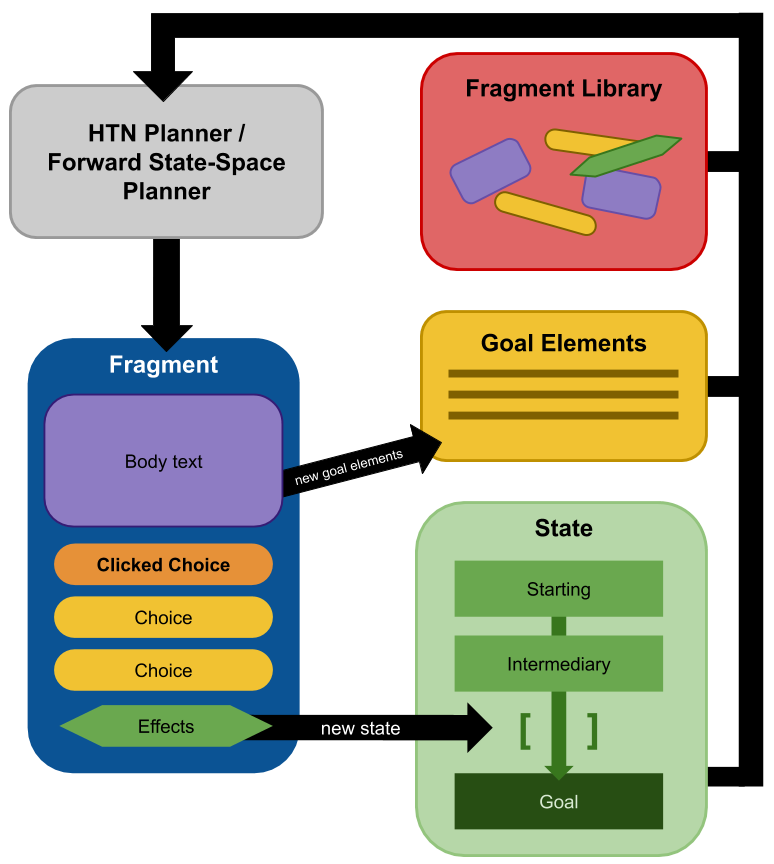
\includegraphics[width=\textwidth]{figures/3-StoryAssembler/storyassembler-system-diagram.png}
    \caption{A flow diagram of the StoryAssembler system.}
    \label{fig:system-diagram}
\end{figure}

\subsection{Core Architecture}
\label{core-architecture}

As mentioned earlier, StoryAssembler's core unit is the ``fragment", which is assembled from component parts in the ``fragment library." It chooses whatever valid combination best results in combined effects that modify the state blackboard to achieve (or make incremental progress towards) the goal state defined by the goal elements (Figure \ref{fig:system-diagram}).

It accomplishes this through two distinct components working in tandem: a forward state-space planner \cite{forwardPlanner} on the highest ``plot-progression" level, and an HTN-like planner  \cite{htn} used for the composition of fragments to accomplish that progression (Figure \ref{fig:htn}). Each StoryAssembler scene has a starting state with initial blackboard values of booleans, strings, or integers, and a goal state, composed of goal elements also represented as blackboard values, such as \texttt{introduceNemesis eq true}.

%%%%%%%% BEGIN FIGURE %%%%%%%%%%%%%%%%%%%%%%%%%%%%%%%%%

\begin{figure}
    \centering
    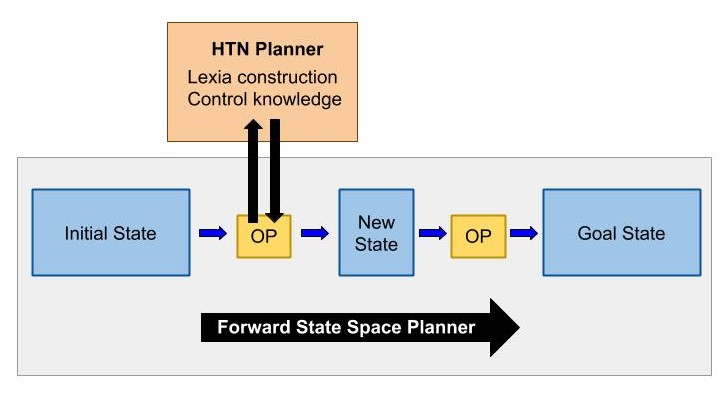
\includegraphics[width=\textwidth]{figures/3-StoryAssembler/htn-diagram.jpg}
    \caption{A simplified flow diagram of how the HTN planner and forward state space planner work together for fragment assembly.}
    \label{fig:htn}
\end{figure}

%%%%%%%%%%%% END FIGURE %%%%%%%%%%%%%%%%%%%%%%%%%%%%%%%%

When executed, StoryAssembler looks at the starting variables' states, looks at the goal state as a list of desired goal states, and then assembles fragments to push it closer to that goal. It does this by recursively searching the library for components---be that body text or choices---to maximize progress towards the goal state. Additionally, it scores fragments higher if they link to other fragments that make goal progress, or incorporate into themselves other fragments that make goal progress as compound fragments. In this way, the search is similar to one done by a hierarchical task network (HTN) planner, where each fragment in the library specifies a set of sub-tasks to pursue (e.g., finding choices or body-text with specific properties). The recursion / look-ahead depth for how many linking fragments are checked for scoring purposes is manually set. For example, in \textit{Emma's Journey}, we found that looking three ``choice-steps" ahead was more than enough to return sensibly-scored assemblages. Anything further may technically return ``better scoring results", but is at (or beyond) the limit of the design skills of authors, given the current tooling and available visualizations (which is discussed in \ref{clarity}).

The final assembled fragment represents the best next ``operation" for the forward state-space planner, and it continues in this manner until the scene ends. In short, StoryAssembler greedily optimizes for fragments that fulfill the maximum number of goal elements, as well as every choice in that fragment going to subsequent fragments that fulfill the maximum number of goal elements, et cetera. While larger questions of hill climbing and getting stuck in local maxima are valid, for us this implementation was sufficient to start tackling the \textit{authorial} concerns around expressiveness and authorial burden, so focus then shifted on how to produce content that could effectively leverage the strengths of this system.

Choice-based narratives are a particularly interesting and fruitful domain for planner-driven narrative systems, due to this additional combinatoric factor in the assembly of choices and displayed framing text. Because the framing text, the choice label, and the destination of the choice link are each their own atomic unit, it means those fragments can combine effects as compound operations, opening up a wide combinatoric space of possibilities. However, it's also these same compound combinatorics that come back to haunt us with challenges to Clarity when authoring content, which we'll expand on later in Section \ref{clarity}.

After the reader selects a choice, the system re-evaluates the current state, looks at the goal state, and re-plans to assemble the next fragment accordingly. Rather than pre-generating possible paths, this ``lazy evaluation'' was chosen because in its initial project (\textit{Emma's Journey}) a mini-game continuously runs in parallel, affecting StoryAssembler's blackboard state. Therefore, it made sense to not evaluate the path forward until the moment of the player's choice, in case an originally valid state was invalidated by gameplay while the text was displayed, or the reverse. 

Additionally, while StoryAssembler operates in this ``live'' mode, it can change displayed text and choices asynchronously in reaction to other game processes, or elapsed time, as detailed in Section \ref{templated-text}'s discussion of text templating.

%%%%%%%% BEGIN FIGURE %%%%%%%%%%%%%%%%%%%%%%%%%%%%%%%%%

\begin{figure}
    \centering
    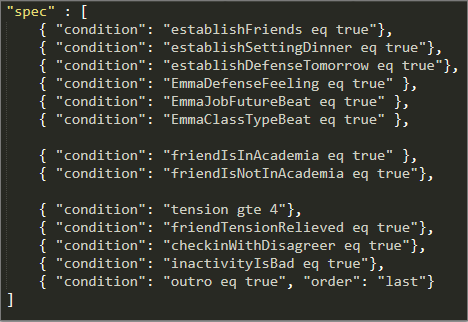
\includegraphics[width=\textwidth]{figures/3-StoryAssembler/story-spec.png}
    \caption{A sample goal state (``spec") detailing dramatic beats to be hit (boolean values) and mood conditions (tension).}
    \label{fig:story-spec}
\end{figure}

%%%%%%%%%%%% END FIGURE %%%%%%%%%%%%%%%%%%%%%%%%%%%%%%%%

\subsubsection{Goal States}

Each scene in StoryAssembler has a corresponding goal state containing a series of goal elements (Figure \ref{fig:story-spec}). A goal element, like blackboard entries, can contain boolean, string, or integer values, and authors may use them for anything from dramatic beats ({introduceFriend eq true}) to mood conditions ({tension gt 5}) or flags to inform the system where the reader has been, or which choices they've made ({complimentedWaiter eq true}). Goal elements can be partially ordered through possession of the optional tags ``first'' or ``last,'' but in general StoryAssembler treats them as an unordered list. The system will end the scene once every goal element has been satisfied at some point in the story (i.e., if a later fragment sets a boolean goal element such that it is invalid, it doesn't ``unsatisfy'' that entry). This design decision was made so that we could have more flexibility in the design of beats within a scene to change the underlying state to multiple values as the scene progressed. For example, if we wanted two characters to increase their \texttt{friendliness} stat after having an argument, we could put two goal elements \texttt{friendliness lt 2} and \texttt{friendliness gt 2} in our goal state. Of course, this also means authors must take care that reconciliation content that increases \texttt{friendliness} has pre-conditions of low \texttt{friendliness}, so that it doesn't prematurely trigger, but it was deemed an acceptable trade-off. This design decision also facilitated splitting up authoring tasks in scenes without reducing Clarity, because authors could focus on their allotted goal elements, and not necessarily worry about other goal elements that may not concern their narrative area.

Goal elements can also be flagged as persistent, which means the system will always prioritize content that satisfies them, but will not evaluate their satisfaction to gate whether the scene ends. This can be used to make the system prioritize repetitive actions, such as a professor calling on students during a lecture, or taking a turn in a conversation. Typically, this strategy is combined with explicit precondition design on fragments for repetitive actions, to control ordering.

A good example of how goal elements work is the first scene of \textit{Emma's Journey}: the night Emma dines with friends before her PhD defense. This scene's goal state (Figure \ref{fig:story-spec}) contains key elements that both communicate setting ({establishFriends eq true}) and initiate the narrative dynamics. The goal state requires two characters to make their cases whether Emma should pursue academia or activism, that the tension in the room passes a certain threshold (via fragments that increment a \texttt{roomTension} variable), and that Emma discusses her own career aspirations. A library of fragments have been authored that can achieve these goal elements in a variety of configurations, which are assembled by the system into a choice-based narrative, and re-shuffled around depending on how the player makes their choices.

\paragraph{Dynamic Goal States}
\label{dynamic-story-specs}

An interesting advanced authoring capability with StoryAssembler is the ability to make goal elements dynamic. This enables techniques such as exposing them to the player as ``scene settings" before the story starts (Figure \ref{fig:parameterized-summary}). For \textit{Emma's Journey}, we implemented this as ``cycling links'' in the scene description. Players can click on the links to change their text values, which in turn affect the goal elements, and the way the scene plays out once they begin. For example, if the player decides to have both friends more critical, the resulting story the planner assembles will have them challenging the player more on their career choices.

%%%%%%%% BEGIN FIGURE %%%%%%%%%%%%%%%%%%%%%%%%%%%%%%%%%

\begin{figure}
    \centering
    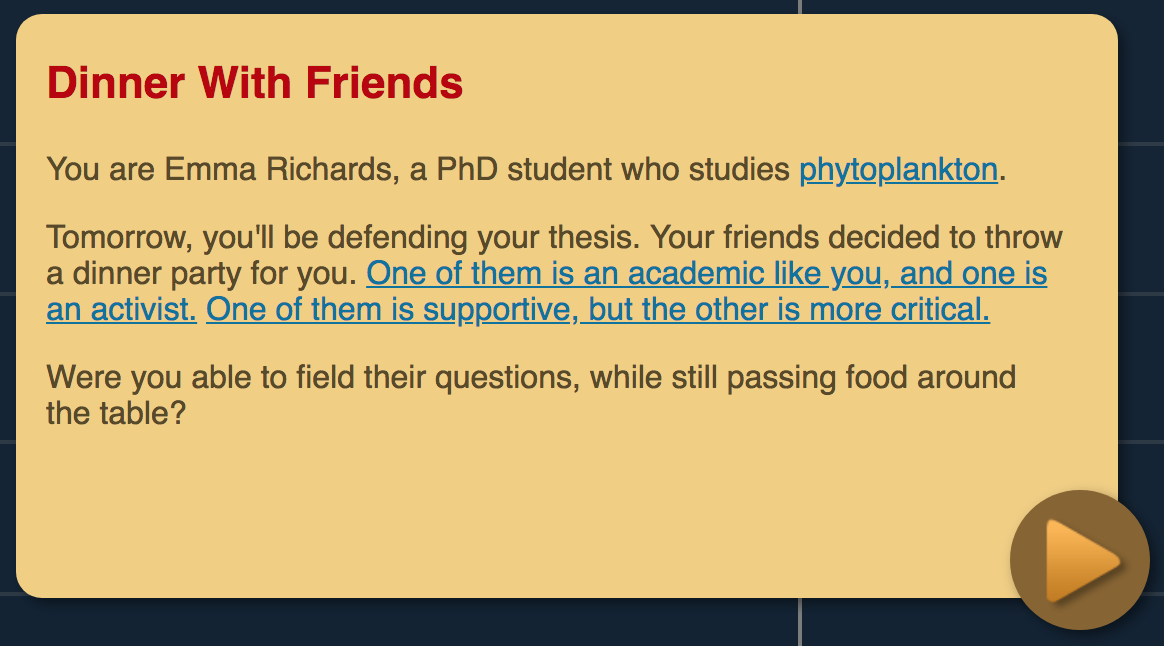
\includegraphics[width=\textwidth]{figures/3-StoryAssembler/parameterized-summary.png}
    \caption{A scene intro, where dynamic goal elements allow players to change friends to be activists or academics, and supportive or critical, as well as Emma's research focus.}
    \label{fig:parameterized-summary}
\end{figure}

%%%%%%%%%%%% END FIGURE %%%%%%%%%%%%%%%%%%%%%%%%%%%%%%%%

In earlier prototypes, this was alternatively exposed as a literal control panel, allowing players to drag sliders around and toggle options on or off. One can imagine this giving rise to several interesting modalities for experiences, and perhaps such controls could even be incorporated into the narrative of the game itself, making them a diegetic way to both surface the capabilities of the system, and deepen the player's engagement.

\subsubsection{Fragment Libraries}

For each scene in StoryAssembler, JSON files of fragments are specified for use. The ability to specify multiple files became a particular asset due to the team-based authoring, as it allowed writers to each use their own file, and substitute placeholder fragments handling other goal elements that other writers were working on. This allowed us to easily develop the game with a sort of rough version control without having to negotiate typical problems with on-boarding such as negotiating merge conflicts, which can be confusing to writers unfamiliar with such systems.

In terms of narrative design pragmatics, this also makes it possible to organize fragment libraries by other features, such as tone, character, or chronology. Or, as in early prototypes of \textit{Emma's Journey}, specify a global library of fragments with highly dynamic, condition-driven text, that could potentially appear within any scene in the narrative. This type of flexibility is similar to what was done in \textit{Ice-Bound} with the level-specific card files, and the global symbol cards file.

\subsubsection{Fragments}

StoryAssembler's core unit of narrative is the fragment. In their canonical form, fragments contain a main section of displayed text (``content"), and a list of choices (``choices"). This is similar to the basic ``passage'' in Twine.

Fragments can also contain pre-conditions to control when they're available. Design-wise, these can be used for causal or temporal ordering. Lastly (and most importantly) fragments can contain effects, which change the state blackboard. This is what is evaluated to determine if the assembled fragment makes progress towards the goal state specified in the scene configuration, and thus drives where and when a fragment will appear. These state modifications can optionally carry through between scenes if authors desire, allowing certain choices to affect later points of the narrative. An example of a fragment data structure can be seen in Figure \ref{fig:sample-fragment}.

%%%%%%%% BEGIN FIGURE %%%%%%%%%%%%%%%%%%%%%%%%%%%%%%%%%

\begin{figure}
    \centering
    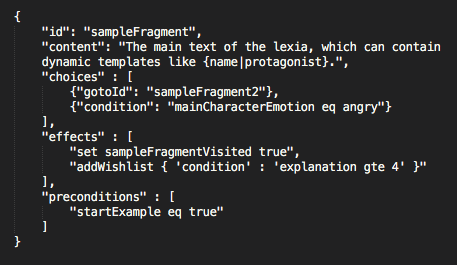
\includegraphics[width=\textwidth]{figures/3-StoryAssembler/sample-fragment.png}
    \caption{A sample fragment showing both static choices (``gotoId") and dynamic choices (``condition") as well as modifying goal elements through effects (``addWishlist").}
    \label{fig:sample-fragment}
\end{figure}

%%%%%%%%%%%% END FIGURE %%%%%%%%%%%%%%%%%%%%%%%%%%%%%%%%

A key capability driving the authorial affordances of StoryAssembler is that fragments can be \textit{compound}, or composed of other fragments. For example, a fragment might contain ``normal" choices (static choice text that directs to another node directly by id) but in place of ``content'' (the main text of the fragment) might instead contain a ``request'' for any valid fragment that increments tension. StoryAssembler then looks for a valid fragment that 

\begin{enumerate}
    \item has effects that increment tension (such as ``tension incr 1")
    \item has a ``content" field with text, but doesn't have choices (ie, it was authored not to stand alone, but to be part of a compound fragment)
\end{enumerate}


It then takes the value in that new fragment's content field, and any effects it has, and combines that with the previous one. The resulting compound fragment would trigger the effects for both of the partial fragments, and would have the body text from the second fragment, with the choices from the first.

Another useful way to think about this is that an assembled fragment in StoryAssembler has three components, each of which uses one of three methods. 

The fragment components are:

\begin{enumerate}
    \item One block of text for ``main content"
    \item A short piece of text for each choice (the ``choice label")
    \item A reference to another assembled fragment visited when the player clicks each choice
\end{enumerate}

Similarly, there are three modes these components can operate in:

\begin{enumerate}
    \item A fragment component can be a non-referential ``string", such as the ``content" field in the Figure \ref{fig:sample-fragment} fragment, which does not reference any other fragment. A fragment can have a string for content and choice label, but a string cannot be used for the choice destination (since by definition it must reference the destination fragment).
    \item A fragment component can be an ``id", which directly links to another specific fragment by its unique id. The first choice in the ``choices" array in Figure \ref{fig:sample-fragment} links to ``sampleFragment2" by id using the ``gotoId" command. All three fragment components can use this mode.
    \item A fragment component can be a ``request", which triggers a search for the most suitable fragment that meets the conditions of the request. The second choice in Figure \ref{fig:sample-fragment} requests any fragment that has an effect setting "mainCharacterEmotion" to ``angry." All three components can use this mode.
\end{enumerate}

Additionally, identical state condition requests can be used for multiple choice destinations, and the system will choose different ``assemblages" to satisfy them, ensuring each choice path is different. For example, one could write a fragment with three choices, two of which increase the tension in the room, and one that alleviates it. StoryAssembler will search the fragment library for unique choice paths that lead to those state changes, and link them in. This enables potentially surprising juxtapositions of paths, and emergent traversals driven by underlying state changes and tracked stats.

While these might seem relatively simple in definition, in practice they can become quite complex, and enable different kinds of narrative experiences. A chart of the different formulations can be seen in Figure \ref{fig:fragment-table}, although many of those remain speculative, given that \textit{Emma's Journey} relied mostly on a handful of formulations, as detailed in Section \ref{implementation-details}'s discussion.

%%%%%%%% BEGIN FIGURE %%%%%%%%%%%%%%%%%%%%%%%%%%%%%%%%%

\begin{figure}
    \centering
    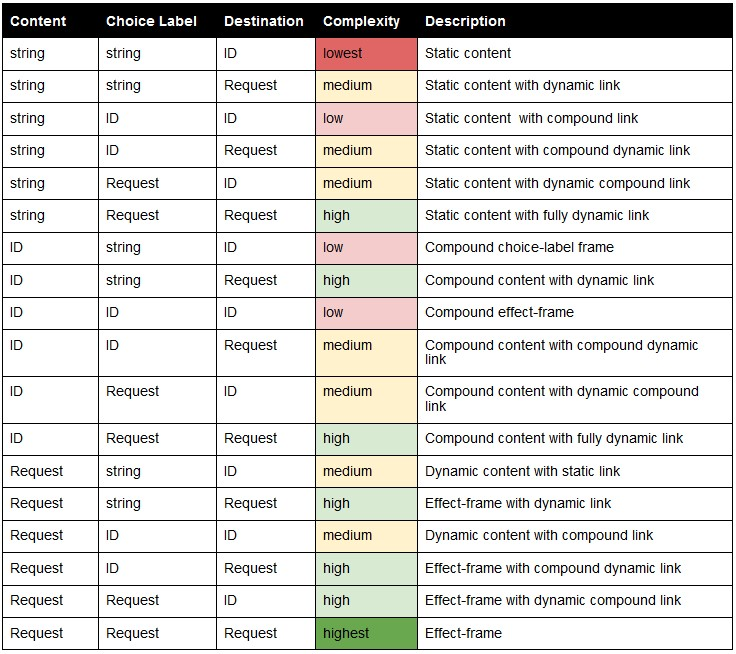
\includegraphics[width=\textwidth]{figures/3-StoryAssembler/fragment-table.jpg}
    \caption{A table of the different StoryAssembler fragment combination methods. Some have somewhat similar affordances (such as ``static content" and ``static content with compound link") and some are quite different. We use ``effect-frame" to designate combinations where the fragment's purpose is to provide a ``frame" for other fragments to be combined within. It has little to no content of its own, but its purpose is a specific content juxtaposition, or addition of its effects to other fragments.}
    \label{fig:fragment-table}
\end{figure}

%%%%%%%%%%%% END FIGURE %%%%%%%%%%%%%%%%%%%%%%%%%%%%%%%%

At the other end of the complexity scale, fragments don't always have to link to other fragments. If no choices are specified in the fragment, the system finds the next best fragment (with valid preconditions) that satisfies the most remaining goal elements, and links to it by creating a ``Continue'' choice. This method frees up authors to author dramatic ``beat'' structures that have internal consistency, but are independently ordered.

In short, StoryAssembler's process is to construct fragments, then evaluate recursively through the choices afforded by the fragment, choosing paths that maximize state changes to fulfill goal elements. In general terms, this means StoryAssembler is always greedily assembling fragments that both contain as many goal-oriented effects as possible, and linking to the most goal-oriented fragments possible. A fragment's effects, choices, and preconditions therefore all play into that process, and must be kept in mind while authoring.

As mentioned before, StoryAssembler can also operate in a ``live'' mode, where at a given interval it re-evaluates the displayed text and choices. If the state has somehow changed while the player was reading the fragment (through an accompanying game mechanic, as with \textit{Emma's Journey}) choices can become unavailable and grayed out, or similarly become available. This affordance can be used to inject urgency into player actions, or make procedurally poignant effects. For example, in a tense conversation with the dean, Emma might lose access to choices to steer the conversation where she wants, if the player's performance in the accompanying mini-game is lackluster. This affordance was added with early Twine works in mind like \textit{Depression Quest} \cite{quinn_2013}, which used the visibility--yet unavailability--of choices as a communicative and persuasive strategy.

\subsubsection{Templated Text}
\label{templated-text}

StoryAssembler's text templates were designed to have similar capabilities to \textit{Ice-Bound}'s. Templates can be used to change the presentation of both fragment content and choice labels. This can be driven by scene state---for example, authors can add hedges like ``umm...'' to dialogue if the state variable ``confidence'' falls below a threshold. This is especially useful when used in tandem with live state modification, as with \textit{Emma's Journey}, where it can signal time-sensitivity to the player, or otherwise communicate the narrative consequences of mini-game performance.

We can also change content more substantially, so that fragments change under different state contexts. For example, we may decide to create a fragment ``complimentHost'' where Emma compliments the host's decor if dinner hasn't started yet, but compliments the food if that fragment is triggered when \texttt{dinnerStarted eq true}. In either case, the fragment's effect to decrease tension is fired, but the text surfacing that is contextual to the current situation.

Templates can also reference character names, pronouns, and other individual mix-ins, so that fragments can be written that are not tied to a specific scene, but rather globally mixed into scenes if their pre-conditions are valid. 

Templates can also be leveraged outside of fragments to have more structural impact. For example, templates can be used in a scene's ``config file", giving authors the ability to cast characters for scenes dynamically, or choose different character qualities before the scene starts that have a perceivable effect on the story. For example, a challenging character can be authored simply as ``antagonist'' and in a previous scene, set as whoever the player escalates a disagreement with. This is gone over in more detail in Section \ref{complexity}'s discussion of Complexity.

\subsection{Emma's Journey}

StoryAssembler was implemented as a JavaScript library. This decision was made due to a couple different factors. One, coming on the heels of \textit{Ice-Bound} (which was entirely built in JavaScript) there was a high degree of comfort with it as a language (the dynamic templating language could be almost directly adapted, functionally speaking). Additionally, the main project driving its development--Emma's Journey--had another component (Gemini) which output Javascript mini-games. The requirement that these two systems talk to each other, and at times modify the state of each other, meant that a common language would be best. While certainly it would be possible to re-implement or ``port" StoryAssembler to another language, its base implementation and feature set was driven mostly through the pragmatics of the project detailed below.

\subsubsection{Implementation Details}
\label{implementation-details}

\textit{Emma’s Journey} is an experimental narrative game that juxtaposes a choice-driven narrative (implemented as a series of StoryAssembler scenes) with a succession of abstract mini-games generated by the Gemini system \cite{Gemini}. It served as a testbed for the development of StoryAssembler and is the first experimental research game to make use of the system \cite{emmaWorkshop}. 

As mentioned in Section \ref{experience-challenge}, the side-by-side presentation of the narrative and generated games is reminiscent of Molleindustria’s ``two-channel narrative game" \textit{Unmanned} \cite{Unmanned}. Players experience a series of scenes from the life of the titular character Emma, initially a climate researcher preparing to defend her PhD dissertation, and make choices that influence the progression of Emma’s career while the world’s climate changes in the background. 

In each scene the player is presented with a single generated mini-game, which interacts with the narrative. We experimented with several different modalities in this project: 

\begin{itemize}
    \item losing the mini-game resulting in a fragment jump in the narrative to a ``losing" path that quickly ends the story
    \item using text templates to change sentences on a word-by-word level progressively as performance worsens in the game for a maintenance task
    \item conditioning choice availability based on game state, making certain choices only available if game performance is good (reminiscent of Quinn’s \textit{Depression Quest} \cite{DepressionQuest})
    \item locking narrative progression to game progression (with no loss condition for the game)
\end{itemize}

In one scene, for instance, Emma is eating dinner with her friends, and the player must play the mini-game to pass food around the table (Figure \ref{fig:gemini-game}). Failure to do so with sufficient frequency will result in the game interrupting the narrative, blocking progression until the player passes the food again. 

In a scene using the ``progression lock", the player must play the mini-game to clean up a beach while holding a conversation with fellow volunteers. The progression of the conversation stops with a ``let's clean up some more" until a checkpoint is passed, which then unlocks the choice to continue. In one of the more difficult scenes, the mini-game performance controls Emma’s concentration during a lecture in front of her class. As the player's performance deteriorates, awkward hedges start appearing in Emma's lecture, ultimately resulting in a narrative failure that ends the scene prematurely if the game is lost. A subsequent scene with the Dean showcases many of these dynamics in unison, as detailed in the following section.

%%%%%%%% BEGIN FIGURE %%%%%%%%%%%%%%%%%%%%%%%%%%%%%%%%%

\begin{figure}
    \centering
    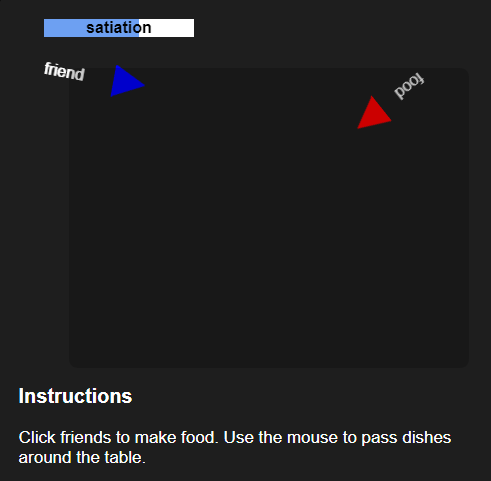
\includegraphics[width=10cm]{figures/3-StoryAssembler/game.png}
    \caption{A Gemini-generated minigame. In this case, the game revolves around passing food around a table.}
    \label{fig:gemini-game}
\end{figure}

%%%%%%%%%%%% END FIGURE %%%%%%%%%%%%%%%%%%%%%%%%%%%%%%%%

Gemini, the system responsible for generating the mini-games that accompany each scene's narrative, is a game generation tool based on what Treanor et al. term proceduralist readings \cite{treanorProceduralistReadings}: interpretations of a game’s ``dynamics, aesthetics, and higher-level meanings" deduced directly from its mechanics, in conjunction with a corpus of cultural knowledge. Gemini accepts as input a file of desired ``readings" or interpretations for the generated game, specified in the form of a logic program, and uses answer set programming to work backwards from these specifications and construct games that can be read in the desired ways. These mini-games have a couple variables that broadcast their values to StoryAssembler, which can then change the displayed fragment, or fragment text, accordingly.

And indeed, some of the most poignant affordances can result from this: a mini-game which requires constant attention as the reader watches Emma’s narration grow increasingly nervous, or confident action choices graying out as the player’s performance in the game lags behind. The trade-off is that StoryAssembler must re-plan at each reader choice, since the mini-game may change the state in the interim before the next click, such that those pathway destinations are no longer optimal or even valid. 

The plot structure of \textit{Emma's Journey} went through many iterations before its release. The scene which showed off the widest array of the system's capabilities in these iterations, however, remained the ``Dean's Office" scene, which occurred third in the final sequence.

\paragraph{Dean's Office}

The Dean's Office scene was third in the progression--after the player had taken Emma through a dinner with her friends, and her first lecture with her students. The player established both her area of expertise and her class dynamics through use of the cycling links that modified the goal state for each respective scene, and were surfaced in fragments during the meeting with the Dean.

%%%%%%%% BEGIN FIGURE %%%%%%%%%%%%%%%%%%%%%%%%%%%%%%%%%

\begin{figure}
    \centering
    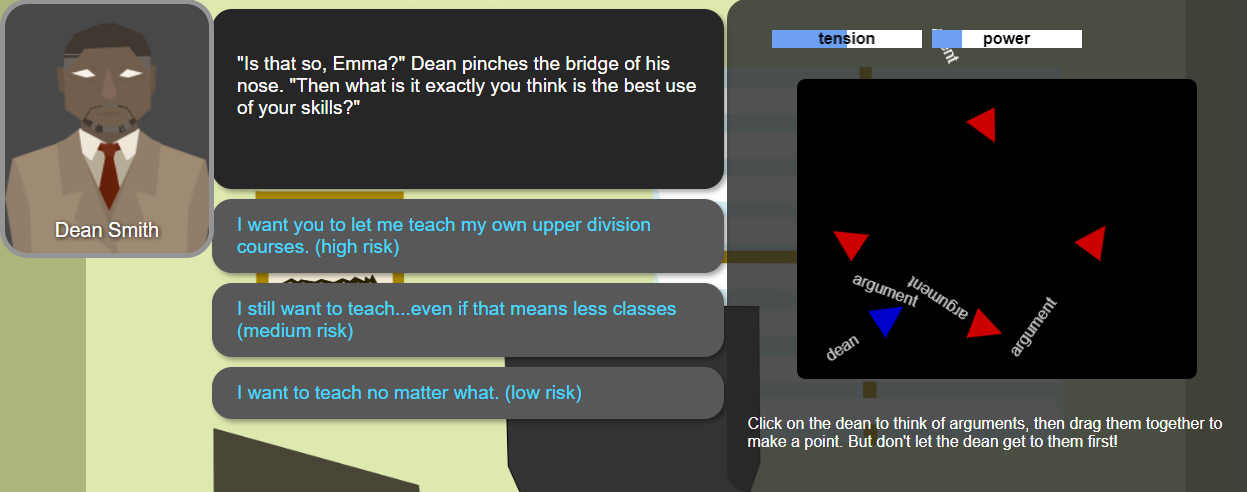
\includegraphics[width=\textwidth]{figures/3-StoryAssembler/dean-level.png}
    \caption{The Dean's Office scene. Here we see the mini-game on the right, which increases power if the player performs well. The choices on the left are labeled ``high risk" to ``low risk." When clicked, they increase the tension, which modifies the game difficulty. Subsequent choices are gated off power values, so poor performance results in not being able to make choices for a good outcome to the scene.}
    \label{fig:deans_office}
\end{figure}

%%%%%%%%%%%% END FIGURE %%%%%%%%%%%%%%%%%%%%%%%%%%%%%%%%

The main dynamic architecture of this scene revolves around whether Emma has succeeded or failed in the previous lecture scene. The lecture scene featured a mini-game that the player could lose, if they weren't performing the maintenance task. Combined with the cognitive overhead of reading a story and making choices, it was easily the most difficult section of the game. If the player had succeeded in the lecture, the Dean would try to pressure them to take on more classes. If they had failed, they would need to justify why they shouldn't be fired.

The Dean's Office has two main variables being tracked: \textit{tension} and \textit{power}. \textit{Tension} relates to whether the scene can finish out to completion (if tension is too high, the scene ends prematurely) and also the difficulty of the mini-game. \textit{Power} is how assertive Emma can be during the conversation to get what she wants (if power is low, conversation options are grayed out and unclickable).

The player can make choices that increase the tension, such as requesting a pay raise or better working conditions. However, if their performance in the game hasn't raised their power enough, when it comes to the choices for giving reasons to justify the requests, they'll be grayed out, forcing the player to capitulate. These values are modified as the game is playing, so may change second-to-second.

Lastly, The Dean’s Office demonstrates on a macro level how scenes can branch based off of conditions in previous scenes. Depending on which ending occurs here, the next scene is dynamically chosen to be either one in which Emma gives a presentation at the UN on climate change for a more ``global effect", or one in which she helps a local non-academic organization relocate an endangered crab species to a new location, for a more ``local effect."

This scene flexed many of the StoryAssembler's interfacing capabilities, and showed how one scene can both have different ways it plays out due to context from previous choices, and can also lead to different subsequent scenes based on the player's choices and performance within that scene.


\subsubsection{Additional Capabilities}

Some capabilities of StoryAssembler were developed, then disabled later on as \textit{Emma's Journey} neared completion. These cuts were made due to pragmatic reasons--sometimes due to difficulties they introduced in content design, sometimes due to feedback from UI usability--but are still interesting to highlight from a system capability standpoint, and as a point of reference for people pursuing similar capabilities.

\paragraph{Global Fragments}
\label{sa-global-fragments}

Initially, we wanted to have a library of global fragments that could be used in multiple contexts within different scenes. It was thought that, if appropriately authored, this could reduce authorial overhead through contextual reuse, without the story seeming to repeat itself. However, in practice it became difficult enough to author fragments that wouldn't seem out of place, that the work involved became greater than if more numerous, specific fragments had been written. As a result, this approach wasn't pursued for \textit{Emma's Journey}. However, the use of multiple content libraries for an individual scene was used to enable multiple authors to work in parallel on the scene, so this capability still exists, just not in the design of \textit{Emma's Journey}. This is elaborated upon in Section \ref{sa-reusability}'s discussion of Reusability.

\paragraph{Dialogue Mode}

For a time we experimented with using a ``dialogue mode" for scenes, which could be set to ``monologue" or ``dialogue" (Figure \ref{fig:discourse-data}). This was then used as an additional scoring heuristic for fragment selection, in the attempt to prioritize fragments that had the correct speaker. This in turn predicated us adding a new field of ``speaker" to every fragment. These values could be statically set to be specific characters, or dynamically determined based on character tags or traits. Speaker fields would be resolved at the beginning of each scene. It was hoped that, since it would position fragments with primary speakers, we could then lean into templated ``mixins" to give them more individual flavor, and add more replayability. It was hoped that if a scene were replayed with different characters cast into different roles, it would feel substantially different, even if the ``bones" of the scene remained the same.

%%%%%%%% BEGIN FIGURE %%%%%%%%%%%%%%%%%%%%%%%%%%%%%%%%%

\begin{figure}
    \centering
    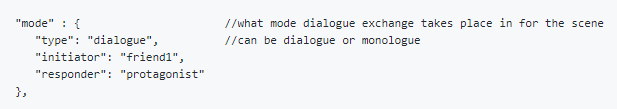
\includegraphics[width=\textwidth]{figures/3-StoryAssembler/data-object-2.png}
    \caption{Data object for discourse mode, here set to ``dialogue" with the character cast as ``friend1" starting off the scene, and the ``protagonist" responding.}
    \label{fig:discourse-data}
\end{figure}

%%%%%%%%%%%% END FIGURE %%%%%%%%%%%%%%%%%%%%%%%%%%%%%%%%

This was simplified out of the library, because after many drafts of content in \textit{Emma's Journey}, it was determined the complexity overhead it added to authoring (See Section \ref{complexity}) wasn't worth the small amount we were leveraging for the story. Additionally, on a narrative design level, it would require adding meaningful differences or changes to the scene story depending on different speakers, and it was hard enough keeping within scope with a static number of characters.

\paragraph{Avatars and Exposed Character Stats}

We did end up using the ``assigned speaker per fragment" design for providing an avatar for whichever character was speaking. These weren't just static images--different avatars for character emotions were created, and then set with value boundaries tied to different state variables. For example, if Emma's confidence falls below a certain threshold while giving a lecture, her avatar changes from a smiling one to a more worried one. The purpose was to provide another avenue to surface the blackboard values to the player (in addition to what was going on with the mini-game) and increase the feeling that the game was reactive and ``listening" to them.

While only one character is shown per fragment in the final version of the game, in early drafts the salient characters for a scene would be shown at the bottom of the screen in a manner reminiscent of RPG characters. Rather than simply binding variable thresholds to control which avatars were shown, multiple values could be bound to single or multiple characters, which would display as ``stat bars" (Figure \ref{fig:lecture}).

%%%%%%%% BEGIN FIGURE %%%%%%%%%%%%%%%%%%%%%%%%%%%%%%%%%

\begin{figure}
    \centering
    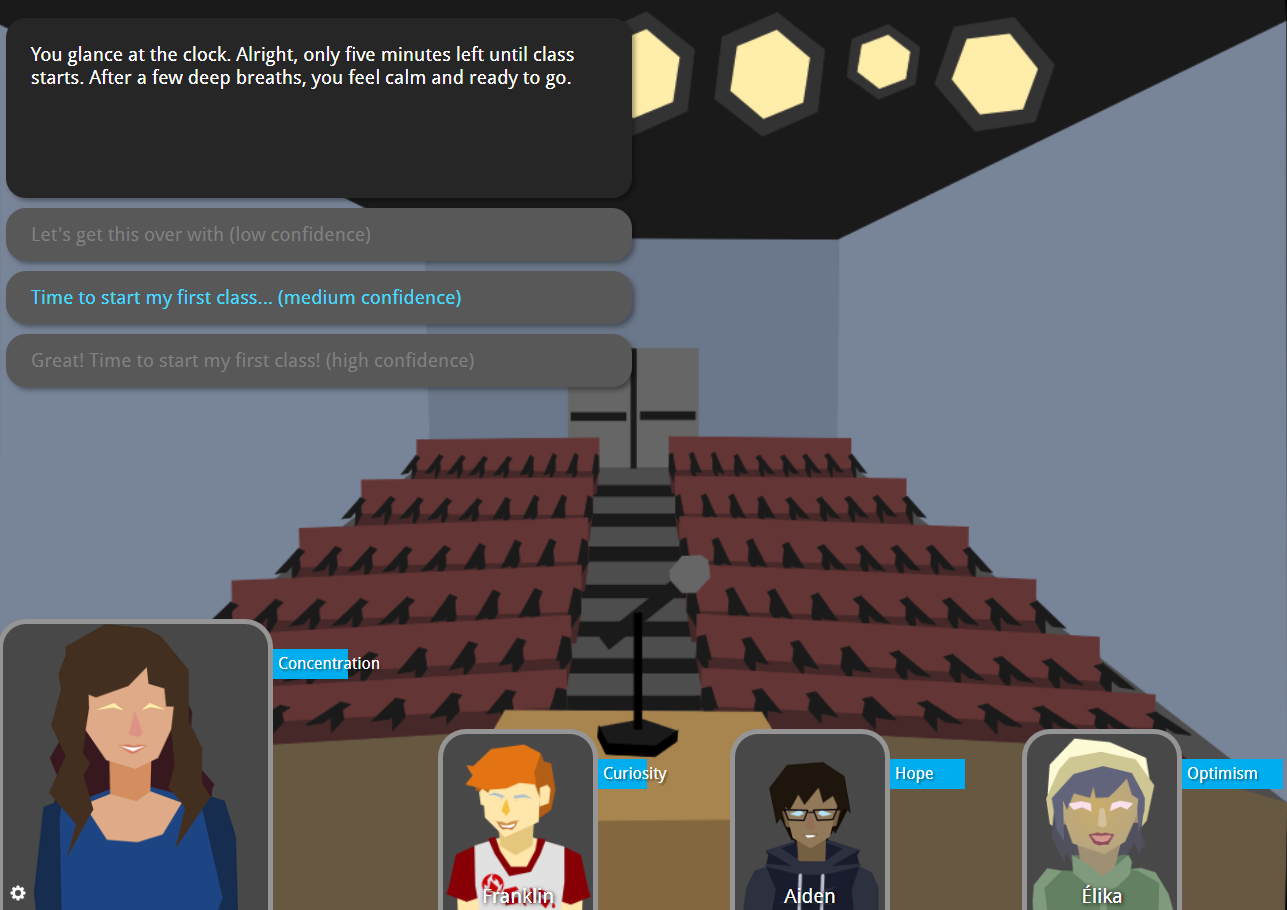
\includegraphics[width=12cm]{figures/3-StoryAssembler/lecture.png}
    \caption{An early prototype, showing state variables bound to characters as ``stat bars" that updated as their values changed.}
    \label{fig:lecture}
\end{figure}

%%%%%%%%%%%% END FIGURE %%%%%%%%%%%%%%%%%%%%%%%%%%%%%%%%

As choices were made with the narrative, players could immediately see how certain choices would change values for other characters, such as ``curiosity", ``hope", or ``optimism." It was hoped that this would help drive home that the choices the player was making were having an effect on the state of the game. After some focused testing with players, however, it was found that the stat bars--when seen in concert with the also-changing mini-game bars--created an information overload, which decreased their utility. Therefore, we made the design decision to only reflect macro-changes through avatar state changes, and keep the mini-game stat bars as the only surfaced qualities the player sees. This made sense for \textit{Emma's Journey}, as most of the scenes where the values were important information were scenes in which the mini-game was the main method used to modify them. However, for possible future games using StoryAssembler, the use of stat bars with characters may prove a useful capability.

\paragraph{Scene Selection UI}

For \textit{Emma's Journey}, two different UIs were developed for scene selection. The first was a scene selection list, where each story scene was placed in a column incrementing through the years (Figure \ref{fig:scene-ui-proto}).

%%%%%%%% BEGIN FIGURE %%%%%%%%%%%%%%%%%%%%%%%%%%%%%%%%%

\begin{figure}
    \centering
    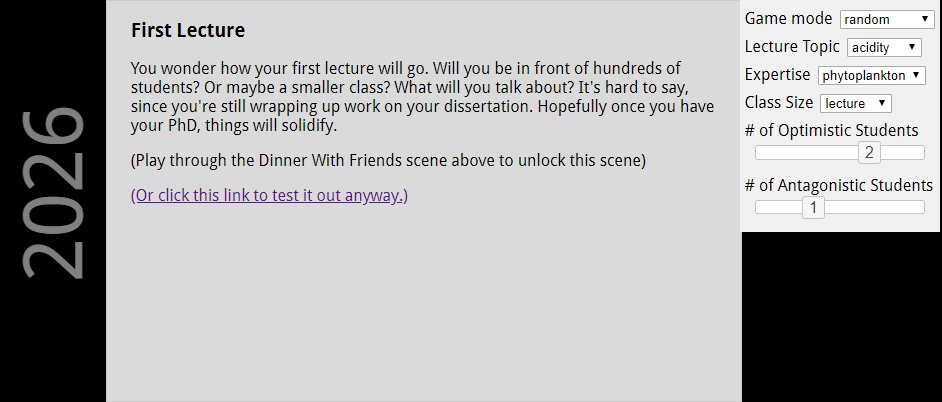
\includegraphics[width=\textwidth]{figures/3-StoryAssembler/proto-UI.png}
    \caption{The ``scene selection" UI layout. Notice the panel to the right. Changing the values here changed parameterized goal elements, driving different priorities for the planner once the scene was begun. This was a less diegetic way of achieving the same effect later realized through cycling links in short scene descriptions.}
    \label{fig:scene-ui-proto}
\end{figure}

%%%%%%%%%%%% END FIGURE %%%%%%%%%%%%%%%%%%%%%%%%%%%%%%%%

When the player clicked the scene, a pop-out control panel on the right would let them set individual scene parameters, which were then sent to the system as modified goal elements. Because the goal state would be different, players could force the system into different formulations for the scene. 

We also experimented with players being able to start a scene at any point in the story timeline, even the last scene first if they wanted! However, the paradoxes of players experiencing scenes out of order, yet wanting to have consequences from earlier scenes affect scenes later in time, meant that we needed to move to a more temporally restricted interface. We attempted having ``bindings" between scene variables, such that players could change variables in temporally earlier scenes to effect later scenes, but in the end it was determined it was too complex an interface for the dynamisms it represented, and we went with a more streamlined appearance.

%%%%%%%% BEGIN FIGURE %%%%%%%%%%%%%%%%%%%%%%%%%%%%%%%%%

\begin{figure}
    \centering
    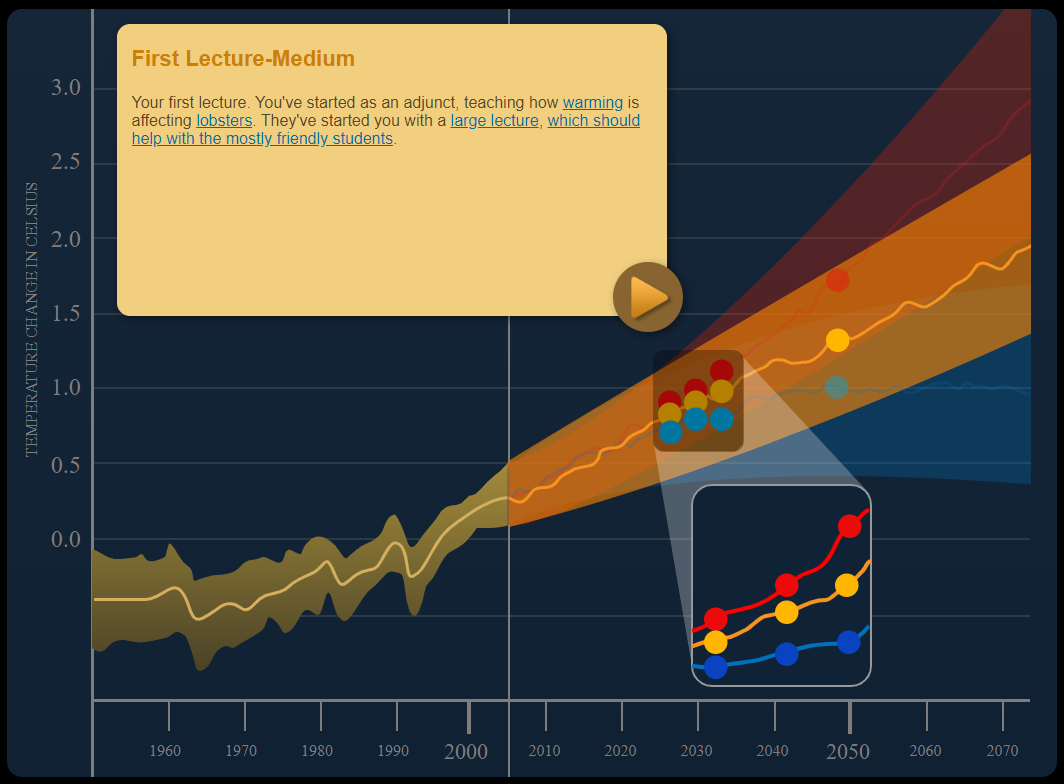
\includegraphics[width=12cm]{figures/3-StoryAssembler/scene-ui.png}
    \caption{Timeline interface for \textit{Emma's Journey}.}
    \label{fig:scene-ui}
\end{figure}

%%%%%%%%%%%% END FIGURE %%%%%%%%%%%%%%%%%%%%%%%%%%%%%%%%

The final interface for \textit{Emma's Journey} was a timeline of the three climate change curves from the \textit{IPCC Report} \cite{ipcc}. The low blue curve represents action taken such that emissions tail off (referred to as the RCP 2.6 curve). The medium yellow curve (RCP 4.5) is if only some action is taken, and the high red curve (RCP 8.5) is if little to no action is taken. At the beginning, the player chooses which line they want to play out. This sets a particular variable for the scenes, which changes some subtle things in the way it is realized. Play then continues scene-by-scene. 

As mentioned earlier, each ``dot" on the timeline has a pop-up paragraph of text with cycling links, which change to new values when clicked. This way, the player can still influence the parameters of the scene, but in a more diegetic way, compared to the previous control panel. Additionally, constraining it to only be traversable in temporal order meant we could side-step potentially confusing the player before they even started playing.

This interface of navigating through a game by traversing a graph is one that has been used in other games as well to emphasize and showcase the choice-driven nature of their narrative, and allow the player to properly appreciate how their decisions scene-to-scene are mapping to the overarching story. For example, the game studio Chunsoft's \textit{Zero Escape} (2012) and its sequel \textit{Zero Time Dilemma} (2016) both prominently feature an interactive flowchart for narrative navigation, allowing the players to choose which scene they play next, or whether they want to replay an earlier segment to get different outcomes and options \cite{mackey_2016}. A screenshot of the ``global flowchart" can be seen in Figure \ref{fig:ref-plot-diagram}. The interplay in that game series between mini-game and narrative is also similar to \textit{Emma's Journey}, in that scenes are predominantly story-based (similar to a visual novel) or game-based (where players have to complete skill-based challenges). Later works like Quantic Dream's \textit{Detroit: Become Human} \cite{dream2016detroit} and Netflix's \textit{Bandersnatch} \cite{bandersnatch} also use this strategy, perhaps as well to show that despite the filmic qualities of the media (that one might then associate with linearity) there are many different paths to the experience, in the hope of foregrounding replayability.

%%%%%%%% BEGIN FIGURE %%%%%%%%%%%%%%%%%%%%%%%%%%%%%%%%%

\begin{figure}
    \centering
    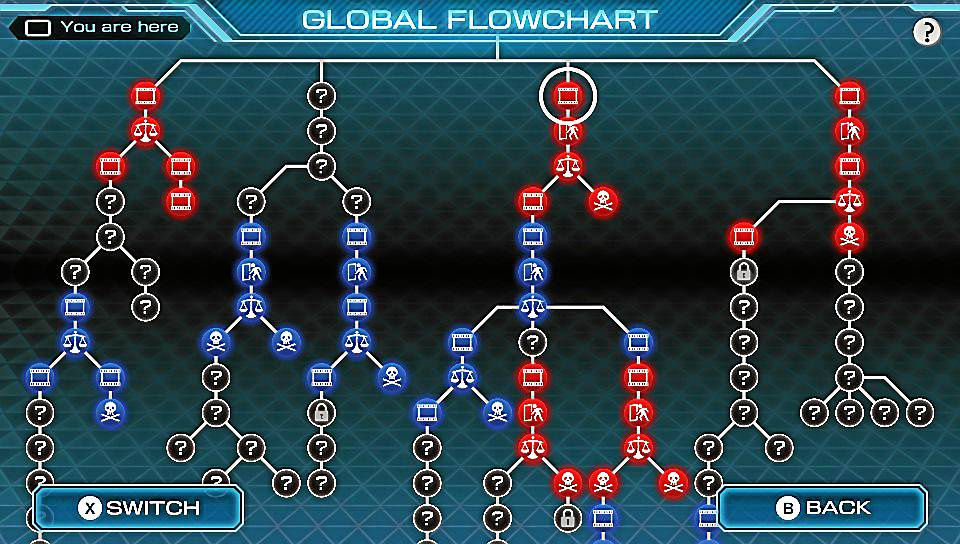
\includegraphics[width=\textwidth]{figures/3-StoryAssembler/ref-plot-diagram.png}
    \caption{Screenshot of the scene selection interface in Zero Time Dilemma.}
    \label{fig:ref-plot-diagram}
\end{figure}

%%%%%%%%%%%% END FIGURE %%%%%%%%%%%%%%%%%%%%%%%%%%%%%%%%

Other games, like \textit{Radiant Historia}, incorporate timeline views as diegetic elements of their story the player accesses and traverses, in this case enabled by a magical book that lets them explore ``Time Nodes" \cite{radiant_historia}. Regardless of diegetic situatedness, this concept of ``exploring different timelines" was something we wanted to employ for \textit{Emma's Journey}, to encourage the player to try different RCP curves and see how the future--and Emma's options--differed.

\section{The Question of Authorial Leverage}

In contrast to \textit{Ice-Bound}, the development of StoryAssembler (and through it, \textit{Emma's Journey}) was much more focused on the development and exploration of new dynamic choice-driven narrative capabilities than the telling of a particular story. For \textit{Ice-Bound}, much of the story was developed up front, and once we had a system capable of telling that story, development of additional system features largely stopped. For StoryAssembler, the exploration of new territory and capabilities was the priority, and we would then see what sort of stories were enabled by them. As such, the story scope and system were under more flux as capabilities were explored, authoring was attempted with them, and they were either reinforced or discarded as infeasible for content production, given the parameters of the project. 

Because of this, \textit{Emma's Journey} has a wide range of Traversability taken across its prototypes, and Authorability for those differed based on efforts made to mitigate the increase in state space and complexity. We will dive into these different states of the project, what we did to try to manage the complexity, culminating in some lessons learned and authoring patterns used along the way.

\subsection{Traversability}

\subsubsection{Explorability}

The entire motivating premise of StoryAssembler revolves around the idea that the content can be dynamically assembled, thus used in a variety of contexts, thus increasing authorial leverage. Ideally therefore, something in the neighborhood of 75\% of authored fragments should be used within a given playthrough of the game, consisting of a complete path through the scenes. In subsequent playthroughs, many of the same fragments might be re-visited, but some different scenes may be triggered due to state differences, driven in part by the state dependency on the mini-game, resulting in a very different outcome.

%%%%%%%% BEGIN FIGURE %%%%%%%%%%%%%%%%%%%%%%%%%%%%%%%%%

\begin{figure}
    \centering
    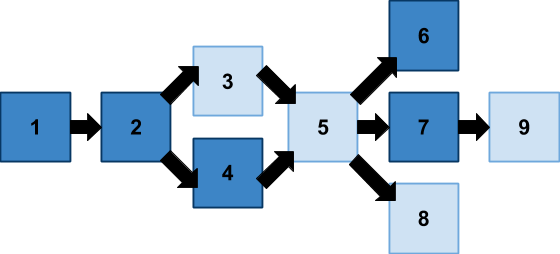
\includegraphics[width=\textwidth]{figures/3-StoryAssembler/plot-diagram.png}
    \caption{A scene-flow diagram for \textit{Emma's Journey}. Light blue squares denote scenes that existed in earlier drafts, but were cut for the final version.}
    \label{fig:plot-diagram}
\end{figure}

%%%%%%%%%%%% END FIGURE %%%%%%%%%%%%%%%%%%%%%%%%%%%%%%%%

Figure \ref{fig:plot-diagram} shows a scene-flow diagram for the intended experience, with lighter squares being ones which unfortunately had to be cut due to time constraints, though they existed as completed StoryAssembler scenes and could be played through in earlier drafts. The goal was to provide both individual variability on the level of the ``choice-trees" constructed in each scene, and from the performance and choices in those scenes, determine which scene would come next.

In terms of how large a state space the narrative is responsive to, \textit{Emma's Journey} was designed with a few key variables for each scene that would vary by a certain amount. When planning out each scene in narrative design meetings, we would make a list of the variables that affected the narrative, the game, and both, and enumerate their dynamics. For example, in Scene 1 (the dinner scene) we track ``confidence", ``enthusiasm for academia", ``tension", and the two friend relationships. Higher confidence opens up more options for Emma to diffuse tension when her friends argue, and her enthusiasm for academia determines which friend dominates the exchange. The tension variable, which rises as the friends disagree, increased the difficulty of the game (in earlier drafts). Enumerating these dynamics early on became critical as authoring progressed for the game, because once the individual fragments were being authored, it would be easy to lose sight of the scene-wide dynamics we were hoping to achieve.

Those were the specific considerations for \textit{Emma's Journey}. In terms of general capability, however, StoryAssembler's state space is left unformalized to the point of being a simple dictionary. Thus, there are no system-imposed limitations on how large a state space stories in StoryAssembler can have. In works like \textit{Emma's Journey}, where it was placed in dialogue with a mini game, the state space could be rather fine-grained (for some levels, we would track multiple values of variables between 0 to 10, whose combinatorics quickly raise that number). However, due to authoring pragmatics, we would ``bin" these values between ranges, and those ranges would typically be simple thresholds to binaries, or three-bin states. Additionally, taking an aforementioned page from Failbetter's book, we tried to hew closely to ``quality parsimony," and use as few variables as possible for these dynamics, in order to make it easier to track state when authoring.

In summary, the types of narrative design StoryAssembler supports and enhances are geared towards context-sensitive and adaptive content, through both the pre-condition logic, and the state-dependent templating that can rework the surface-level text of fragments to preserve coherency if displayed in different situations. Therefore, by implication, the types of games it enables should lean from medium to high explorability, in order to leverage these strengths.

\subsubsection{Replayability}

For \textit{Emma's Journey}, it was hoped that the player might play through multiple times, to experience the difference of the three climate timelines, or make different choices in the scenes. After all, even if interesting choices exist, players may also wonder about branches they haven't explored, which could potentially set us up with issues of repetition for replayability. However, the main focus was on variability and reactivity within the fragments themselves, with a couple hooks present to change which scenes would be activated next. The design implications of this were that we needed to surface the dynamism of the system to the player as we went, as we wouldn't rely on subsequent playthroughs or going back to a previous scene to showcase the variance of fragments. Because the partnered mini-game interaction provided a way to modify the fragments live, this was something we could lean into, as opposed to hoping a subsequent playthrough might get the player into a different situation. However, that still set us up with a requirement of medium to low Replayability, specific to \textit{Emma's Journey}. This de-prioritization is in contrast to \textit{Ice-Bound}, whose centering on the idea of ``sculptural narrative" meant that it was critical to keep replayability, though both still also demanded high explorability.

However, as a general rule, StoryAssembler should be able to support experiences with a very high degree of replayability. Because fragments are state-driven through their pre-condition logic and can have context-dependent content changes through state-based templating, they can (and should) be designed for replayability. This could be pushed further if the narrative design required it. Whether that took the form of repeating individual scenes multiple times between a single playthrough, or doing multiple playthroughs of the entire scene set, an important strategy for ``cashing out" the extra authoring effort for dynamic fragments is to make it possible for different deployment in subsequent playthroughs. Additionally, the goal elements that drive StoryAssembler can be made dynamic, and those controls exposed to the player (as was done with \textit{Emma's Journey}). This could be pushed as a focus for an experience as well, where a player could experiment with modifying the goal state of the scene before entering it, with different fragments being selected to satisfy this changing goal state playthrough-to-playthrough. Managing the combinatorics of changing goal elements, however, would then become the dominant challenge for such a work.

\subsubsection{Reusability}
\label{sa-reusability}

For \textit{Emma's Journey}, we didn't focus as much on fragments appearing multiple times in the same playthrough, but rather dynamic assembly for a single playthrough. Outside deliberate repetitions of content (such as returning to a base fragment where Emma reads an article each time, and it only exits after three articles are read) not many fragments are repeated. This emerged mostly from the fact that authoring with StoryAssembler was already quite complex, and incorporating fragments that would need to show up and have their effects run multiple times through the experience proved too challenging. 

As mentioned earlier in Section \ref{sa-global-fragments}, in early attempts we experimented with ``global fragments", in the hope that generating a wide swath of content, capable of instantiation in any scene, would eventually decrease the difficulty of authoring new scenes, or at the very least start raising the generativity of the narrative across the board. After all, a similar approach had been used in \textit{Ice-Bound}, with good results! However, we found in initial experiments that the differences between a global symbol or event in \textit{Ice-Bound}, and a global fragment in StoryAssembler, were great.

Symbols, events, and endings in \textit{Ice-Bound} are more \textit{discrete} as content units, and structurally, the type of narrative we set out to create with it was centered around that self-containment. We leveraged the ``fires in the desert" modality discussed in Section \ref{subsubsec:failbetter-and-qbn-systems}--where players see a series of scenes, and infer their connections--to avoid difficult problems of connecting content closely together. In contrast, \textit{Emma's Journey} centers around \textit{continuous} content units, where one fragment is connected to the next via a choice. This already presents a difficult problem with the ``choice label" given different contexts. Even more difficult, \textit{Emma's Journey} features conversations as the main focus of scenes, and the \textit{types} of conversations happening in different scenes are not concomitant. Conversation modes may range from talking with two friends, to giving a lecture and answering student questions, to defending against probing questions from the Dean, to having a low-key conversation with a co-worker while cleaning a beach, or parrying confrontational provocations from a corporate interest representative at a UN talk.

Some efforts were made to bridge these differences through the addition of some new syntax and systems. We added the ``Dialogue Mode" capabilities to StoryAssembler primarily because it was hoped that, combined with the use of custom templates per character, we could constrain the appearance of fragments (or composite parts incorporated into other fragments) to situations where the manner of conversation matched up, and then rely on the surface text templating to customize that text to something sensible. In practice, however, the task of conforming the scenes to particular dialogue modes introduced difficulties, and by the time particular fragments were customized to be interchangeable, the complexity of writing them put the time commitment higher than if we'd simply written targeted fragments for each case. 

Thus, due to these \textit{content} commitments for \textit{Emma's Journey}, we decided to move away from using global fragments. As a general rule, however, StoryAssembler greatly facilitates content reusability, whether that's through fragment or scene-level cases. One could imagine a work written with this system where each fragment is instead a short scene, and is more self-contained, perhaps with more generalizable choices that more resemble planner actions (pick up lamp, move to livingroom, etc). Then it would be far easier to incorporate global fragments without running into these \textit{non sequitur} issues. Or perhaps the goal state could be modified such that a given goal element like ``tension eq 5" could happen in different scenes depending on what choices are made, and thus similarly content could be designed to be reused in different scenes where tension-raising fragments were needed. Regardless of the case, StoryAssembler's state-driven templating system means that we can write fragments that display different text when they're repeatedly visited, making fragments feasible across different contexts, or even repeatedly visited ones. However, all of these capabilities come with their own authorability issues that must be kept in mind, which are detailed in the Authorability section.

\subsubsection{Contextuality}

For \textit{Emma's Journey}, it was important that the way fragments were assembled was contextual and made sense as a unified flow from goal element to goal element, while also honoring the player's decision. Especially in choice-driven narratives, a player expects their agency to shape the path through the story, and they can be sensitive to feelings of being ``railroaded" or forced into situations they make choices to avoid. Indeed, the whole affordance around making ``inactive choices," that are shown but can't be clicked, derives its power from displaying the ability to control the narrative, which is then withheld from the player. Therefore, the narrative needs a high level of contextuality to show that it's ``listening" to the player's choices. Compared to \textit{Ice-Bound}, which is more about presenting areas of \textit{possibility} and which can rely on the player to fulfill contextuality through their own ``editorial efforts" (the conceit of the framing story), \textit{Emma's Journey} needed to close that gap on its own. Additionally, the interaction with the mini-game meant that, as much as possible, fragments should change to surface changing game state. As mentioned previously in Section \ref{implementation-details}, specific narrative mechanics such as changing surface text, changing choice availability, or progressing to different fragments automatically, all could happen based on mini-game state.

Because these capabilities are so central to StoryAssembler, it could be generalized to say that all StoryAssembler narratives are setting up an authoring task requiring very high levels of contextuality, and thus care and consideration should be taken for the state space, in order to not inadvertently over-scope.

\subsubsection{Summary}

Thus in summary, the narrative design of \textit{Emma's Journey} was setting us up for the following authorability challenge:

\begin{itemize}
    \item \textbf{Medium Explorability}: While we wanted players to be able to potentially explore the states through the mini-game, due to the choice-based nature of the narrative, not too much explorability is possible in a given playthrough.
    \item \textbf{Medium Replayability}: the three provided climate graphs beckon for replays, as well as the changeable scene introductions which alter the scene goal elements, but the main message of the game--and the main points of research we wanted to pursue--could be satisfied with a single playthrough (though the game would support multiple playthroughs).
    \item \textbf{Low Reusability}: initial drafts and experiments with global fragments proved too complex and labor-intensive for the benefit they provided, given the range of conversational tones within the game. While one could consider each potential narrative path that shares a fragment a ``reuse" of it, the number of different paths was still relatively low, for reasons expanded on in Section \ref{complexity}'s discussion of Complexity.
    \item \textbf{Very High Contextuality}: the demands of our narrative--conversations between characters in very different modes--meant fragments needed to have very high contextuality to fit into the flow and not seem like non sequiturs. It also needed to reflect the player's choice, and react to changing mini-game state, potentially in a live manner.
\end{itemize}


 


Emma's Journey was a narrative design challenge on many fronts, which stretched our capabilities in many ways as we explored different narrative and system dynamics. Our goal was a lofty one, and though by the end compromises needed to be made in order to finish the experience, many valuable lessons were learned across the three main categories of Authorability.

\subsection{Authorability}

Having established the authoring challenge set to us by the experience we wanted to provide through \textit{Emma's Journey}, we can talk in a detailed and structured manner about how authoring with StoryAssembler works, and the pragmatics of content creation for this motivating game. As before, we'll start with Proficiency, detailing our process of working with a team of novice writers to create content for the game, and how we sought to amplify and support their efforts. Next, we'll talk about Complexity, and dive into the deep details of what writing a scene with StoryAssembler entails, from both a narrative design standpoint and a technical standpoint. Last, we'll talk about StoryAssembler's biggest stumbling block: Clarity. We'll walk through the challenges we faced trying to surface the system dynamics to authors, some of the strategies we used to mitigate it, and compromises we were forced to make.

\subsubsection{Proficiency}

StoryAssembler requires authors write fragments as JSON objects. This format was chosen because JSON is a very well-supported and abstracted format, that has third-party tools already created to help write it. For \textit{Emma's Journey}, we had our writers use a free, off-the-shelf code editor (Sublime Text) which comes with highlighting for malformed JSON.

We also used a library called HanSON (\url{https://github.com/timjansen/hanson}), which allowed us to add comments to our JSON files. This proved critical not just so that others looking at files could understand what a particular fragment or group of fragments accomplished, but for the authors themselves to organize and tag different fragments with what they should be accomplishing.

JSON as a format is fairly forgiving--with some content parsing passes to make syntax error messages more understandable and specific, we got to a point where most of the writers were comfortable writing with it, and could produce content relatively quickly.

It bears mentioning that, for \textit{Emma's Journey}, we had a ``proficiency case" closer to that which is the norm for non-academic projects. As opposed to \textit{Ice-Bound}, where the only content creators were the same people developing the system, \textit{Emma's Journey} was collaboratively authored between a team of undergrad writers, and some peer collaborators. The bulk of the writing done for \textit{Emma's Journey} was undertaken by novice writers, some of which were unfamiliar with even Twine as a writing tool. Thus, while initially it was thought that we could potentially drastically increase our ability to produce content for the game (and quickly move into territories where the system, having a greater library of content to select from, would start to show some procedural muscle) it turned out more focus needed to be given to support our writers in those goals.

There is also a Proficiency issue that similarly afflicted Spierling and Szilas with authoring for their IDtension and Scenejo systems. Namely: the system was still being developed while authoring was underway, and features might be added or changed as requirements for the project and scope changed. While Spierling and Szilas noted ``it is necessary that both lines develop in co-evolution" (which we similarly hold true) ``there is a vicious circle at the beginning of this co-evolution, as there are mutual dependencies between the two actions [...] we cannot expect that newcomers as authors in Interactive Storytelling provide us with proper specifications of their needs, when they still cannot grasp the potential offered by engines and by the medium" \cite{authoring_issues}. As an extension of this, the changing nature of the system and experience meant that our authoring team's Proficiency would be ``reset" or lowered, as new features were added that they were expected to use in their writing.

Proficiency also isn't necessarily limited to technical proficiency, or even systemic narrative design proficiency. We also needed to overcome project management challenges in dividing up content creation responsibilities, and in order to do that, long design meetings needed to happen on a frequent basis, in order to provide consensus on the systemic dynamics each scene would need to show, and how those would interact with the mini-game. Thus, an important lesson learned here was that providing not just technical support, but structural support for writers when working in groups to create content for one's system, was a significant amount of effort that needed to be planned for.

\paragraph{Authoring Tool}

While JSON is a relatively friendly syntax to author in, we wanted to make things even simpler. Small mistakes, like forgetting to put a comma between properties in a data object, could result in unintuitive error messages that could take time to figure out, and pop the writer out of ``writing mode" and into ``syntax troubleshooting" mode. Additionally, the presence of syntax errors in another person's file, if they committed it (a practice we did our best to discourage) could wrongly give the impression a person's fragments were malformed. To try and mitigate this (and to try to head off other issues) we attempted a rough pass at creating an authoring tool.

To accomplish this, we adapted code from a library called ``JSON Editor" (\url{https://github.com/json-editor/json-editor}) to work with StoryAssembler fragments. This allowed us to quickly create a clear and uncluttered GUI that eliminated the problem of forgotten commas, etc. However, we traded one set of problems for another: we found ourselves trying to thread the needle between displaying as much information as possible on the screen, and keeping the interface clean and intuitive to use. Because of the high referentiality of fragments between each other, it was important to be able to see many at once, in order to compare different values for combination. Also, while having a GUI gets rid of input errors, it also makes that most critical of systemic writing tools--text search--a complex problem to deal with.

We were able to spin up a tool relatively quickly using the aforementioned libraries, and it worked well for simple cases of StoryAssembler authoring. However, the sticking point which ultimately led to our abandonment of it, was that various edge cases--such as various classes of compound fragments--were prohibitively difficult to modify the library to handle. What made this problem even more pernicious was that it was exactly these types of cases that were the most procedural, and therefore most in need of tool support. Rather than split the authoring paradigm between a GUI for ``simple" cases and a code editor for ``complex" cases, we opted to continue with the unified approach using Sublime Text.

\subsubsection{Complexity}
\label{complexity}

StoryAssembler can be a simple system to work with. One could use it to write static hyperfictions, identical in form to Twine works, relatively easily. But in practice this would be like using a rather complex Rube Goldberg machine to butter toast. Given the high amount of support for complex dynamisms, it is incumbent on authors choosing to use such a system to push its limits. Certainly, the framing of its creation for \textit{Emma's Journey} was one in which we were trying to push it as hard as possible, adding capabilities as we went to explore how that impacted authorability and the generation of the narratives. Thus, StoryAssembler as a rule is a has high Complexity. This stems primarily from the richness of its capabilities, and the number of different narrative design strategies it can accomodate. In order to understand this fully, we need to take a close look at the authoring process for a scene, and a fragment within it.

StoryAssembler narratives are comprised of scenes, one or many in sequence. Which scene follows another can be statically determined, or dynamically assigned via state in the previous scene. To create a scene, authors must complete two main tasks: constructing a scene's goal state, and authoring content that fulfills it. In terms of authoring pragmatics, this typically means a back and forth between authoring of the goal state--a list of goal elements--and fragments which can be assembled to fulfill them.

By the time we hit our stride authoring content for \textit{Emma's Journey}, our process for authoring a scene would go through a series of stages. First among those stages was a rough outline of the type of story we wanted to tell in more abstract terms. ``Emma has a disagreement with her friends over dinner" or ``Emma has a challenging first lecture." We would also have a list of qualities we wanted the mini-game or the narrative to influence. Then we would construct the ``beat clusters" of what we wanted to happen in the scene, and what ordering constraints (if any) they had. These ``beat clusters" would then be reified into goal elements, which we would then put into the scene's goal state. For \textit{Emma's Journey}, a typical scene would have roughly fifteen goal elements in its goal state, and around fifty to seventy-five fragments.

Before you can write fragments to fulfill the goal elements, though, you need to set up the scene config file. This is quite an involved process, that also requires some planning in advance. The list of required components is displayed in Figure \ref{fig:scene-components}.

%%%%%%%% BEGIN FIGURE %%%%%%%%%%%%%%%%%%%%%%%%%%%%%%%%%

\begin{figure}
    \centering
    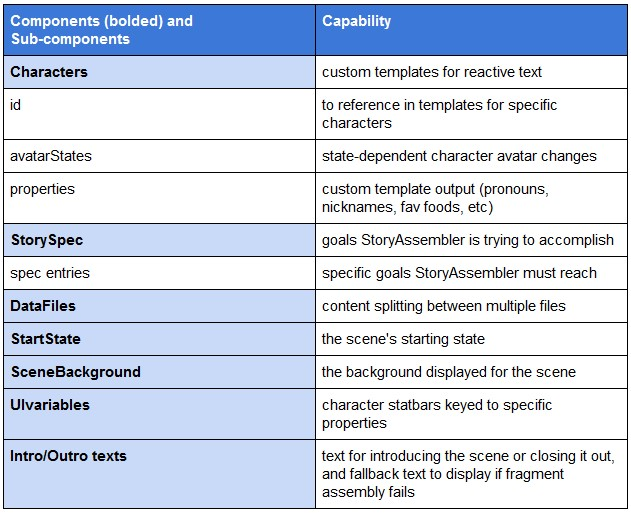
\includegraphics[width=\textwidth]{figures/3-StoryAssembler/scene-components.jpg}
    \caption{A list of required components for a StoryAssembler scene.}
    \label{fig:scene-components}
\end{figure}

%%%%%%%%%%%% END FIGURE %%%%%%%%%%%%%%%%%%%%%%%%%%%%%%%%

Some of the most critical info in this, namely the goal state, requires that writers plan out their scene before committing to writing content for it, as we did for \textit{Emma's Journey}. Unlike authoring systems like Twine or Ink, this sort of up-front narrative design can stifle creativity initially, but hopefully as scene writing continues and the goals are fully fleshed out, experimentation with creative ways to achieve said goals can provide fertile ground for writers. This is similar to our experience writing for \textit{Ice-Bound} under thematic constraints towards the end of content creation, and also echoes some of the constrained writing practices from Oulipo. Obviously, the information encoded in the config file is subject to change as the scene evolves, although the more elaborate the goal state, the more ``finicky" changing goal elements could be, resulting in ``unhappy accidents" where the system would be unable to bridge to necessary choice branches, due to pre-conditions or effects not firing in the same way.

Once the planning was done and the goal state filled out, we could move on to fragment authoring. This also could become quite complex, as more features were added to the system that resulted in additional fields needing to be written and accounted for in subsequent fragments. A list of all fragment components can be seen in Figure \ref{fig:fragment-components}.

%%%%%%%% BEGIN FIGURE %%%%%%%%%%%%%%%%%%%%%%%%%%%%%%%%%

\begin{figure}
    \centering
    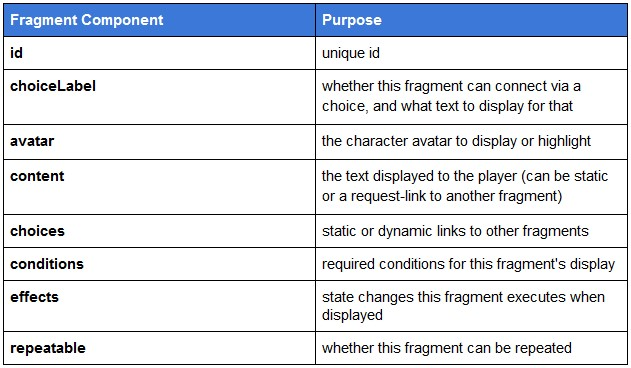
\includegraphics[width=\textwidth]{figures/3-StoryAssembler/fragment-components.jpg}
    \caption{Fragment components.}
    \label{fig:fragment-components}
\end{figure}

%%%%%%%%%%%% END FIGURE %%%%%%%%%%%%%%%%%%%%%%%%%%%%%%%%

In \textit{Ice-Bound}, there was a sense while writing that one could start with static, simple content, then add the dynamism as you went along. That way the system would get progressively more dynamic, but you would always have a ``fallback." You wouldn't fail, just successfully work with less than the desired dynamism. Common sense dictated that a similar strategy might work with \textit{Emma's Journey}.

However, we found that the difference between the simplest formulation--that of the static link fragment with string body text and choice label--did not ``play well" with more dynamic fragments (as detailed in the next section). In the end we pushed as much dynamism as we could get and still ensure a playable narrative experience, but these difficulties with the incremental addition of dynamic content meant that there were still far more static fragments in the final project than we originally intended. Our ideal fragments, composed of several interchangeable sub-fragments, remained more ``hero" content creation than anything. A diagram of a hypothetically ``maximally dynamic" fragment can be seen in Figure \ref{fig:maximal-components}.

Even if a fair number of \textit{Emma's Journey} fragments themselves were static, however, there was still the state-driven templating aspect that could change their surface text, and even statically linked fragments could be ``dynamically triggered" if they depended on parameterized goal elements, and then exposed in the scene description for the reader to change. Thus, while falling short of our initial expectations for dynamism, there was still plenty left to surprise us, given these other affordances.

%%%%%%%% BEGIN FIGURE %%%%%%%%%%%%%%%%%%%%%%%%%%%%%%%%%

\begin{figure}
    \centering
    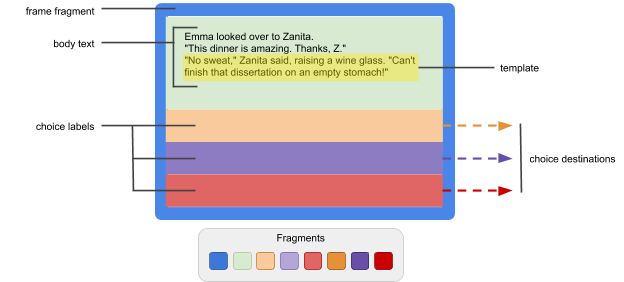
\includegraphics[width=\textwidth]{figures/3-StoryAssembler/fragment.png}
    \caption{An example 3-choice StoryAssembler fragment with eight different fragment references (a frame fragment, body text from a fragment, three choice labels and three choice destinations, each to unique fragments).}
    \label{fig:maximal-components}
\end{figure}

%%%%%%%%%%%% END FIGURE %%%%%%%%%%%%%%%%%%%%%%%%%%%%%%%%

Regardless, planning the goal state and writing the fragments to fulfill it involved a high amount of Complexity. The aforementioned issues with unintended side effects, while a product of the content creation complexity, play into StoryAssembler's most dogged authorability challenge: Clarity.

\subsubsection{Clarity}
\label{clarity}

Because of all the components required for both goal elements and individual fragments, reaching high Clarity for authors using StoryAssembler can be a stiff challenge. Because the baseline unit of content for StoryAssembler is the fragment, finishing a story ``beat" frequently, if not always, requires writing multiple fragments (not to mention the additional fragments required if one wants to provide choices, which is the point of the whole system!). This means that, when writing for StoryAssembler, the dynamics of how content is selected can never be far from the writer's mind. This is in contrast to systems like \textit{Ice-Bound} or Delve, where the individual units of content are more self-contained. This is reflected in their lower Contextuality score, and is directly tied to author's ability to author for them in a more isolated, standalone fashion.

\paragraph{Data Visualization}

As with \textit{Ice-Bound}, one thing which can greatly increase Clarity for authors is data visualization. This allows them to get a sense of what shape the story is taking, and what content needs to be authored to fill gaps in coverage.

Without a tool, the only way to double-check content authoring in StoryAssembler works is through exhaustive traversal of the choices. Due to their dynamic assembly, this means the entire structure must be re-verified with each added fragment or choice, to ensure a changed or added fragment isn't showing up in an undesired spot due to unforeseen state conditions.

Therefore, the visualization solution created for StoryAssembler needed to show three things: the assembled choice structure, when goal elements were being fulfilled, and how content was being re-used. Given that the code underlying StoryAssembler was under active development, we got our data by running a ``headless" version of the scene, and automatically traversing it. This meant that the code running for the visualization was the same as what ran the game, and changes to the engine as it was developed were always faithfully reflected in the visualization. 

The viz tool would traverse the structure in a depth-first manner, keeping a list of the choices it had not yet visited as unique entries of ``clicks" on the UI from the beginning of the scene. When it reached the end of the scene, it would go to the array, run the clicks of the next entry, and proceed from there. In the case of ``no path found" errors, it would flag that data to be represented as an error.

The resulting data was displayed as an interactive directed graph using the Cytoscape.js library \cite{cytoscape}. We chose this library because it comes with built-in graph traversal and layout algorithms, which streamlined some of the development. In addition to graph layout, other strategies were used to expose some of the underlying structure.

%%%%%%%% BEGIN FIGURE %%%%%%%%%%%%%%%%%%%%%%%%%%%%%%%%%

\begin{figure}
    \centering
    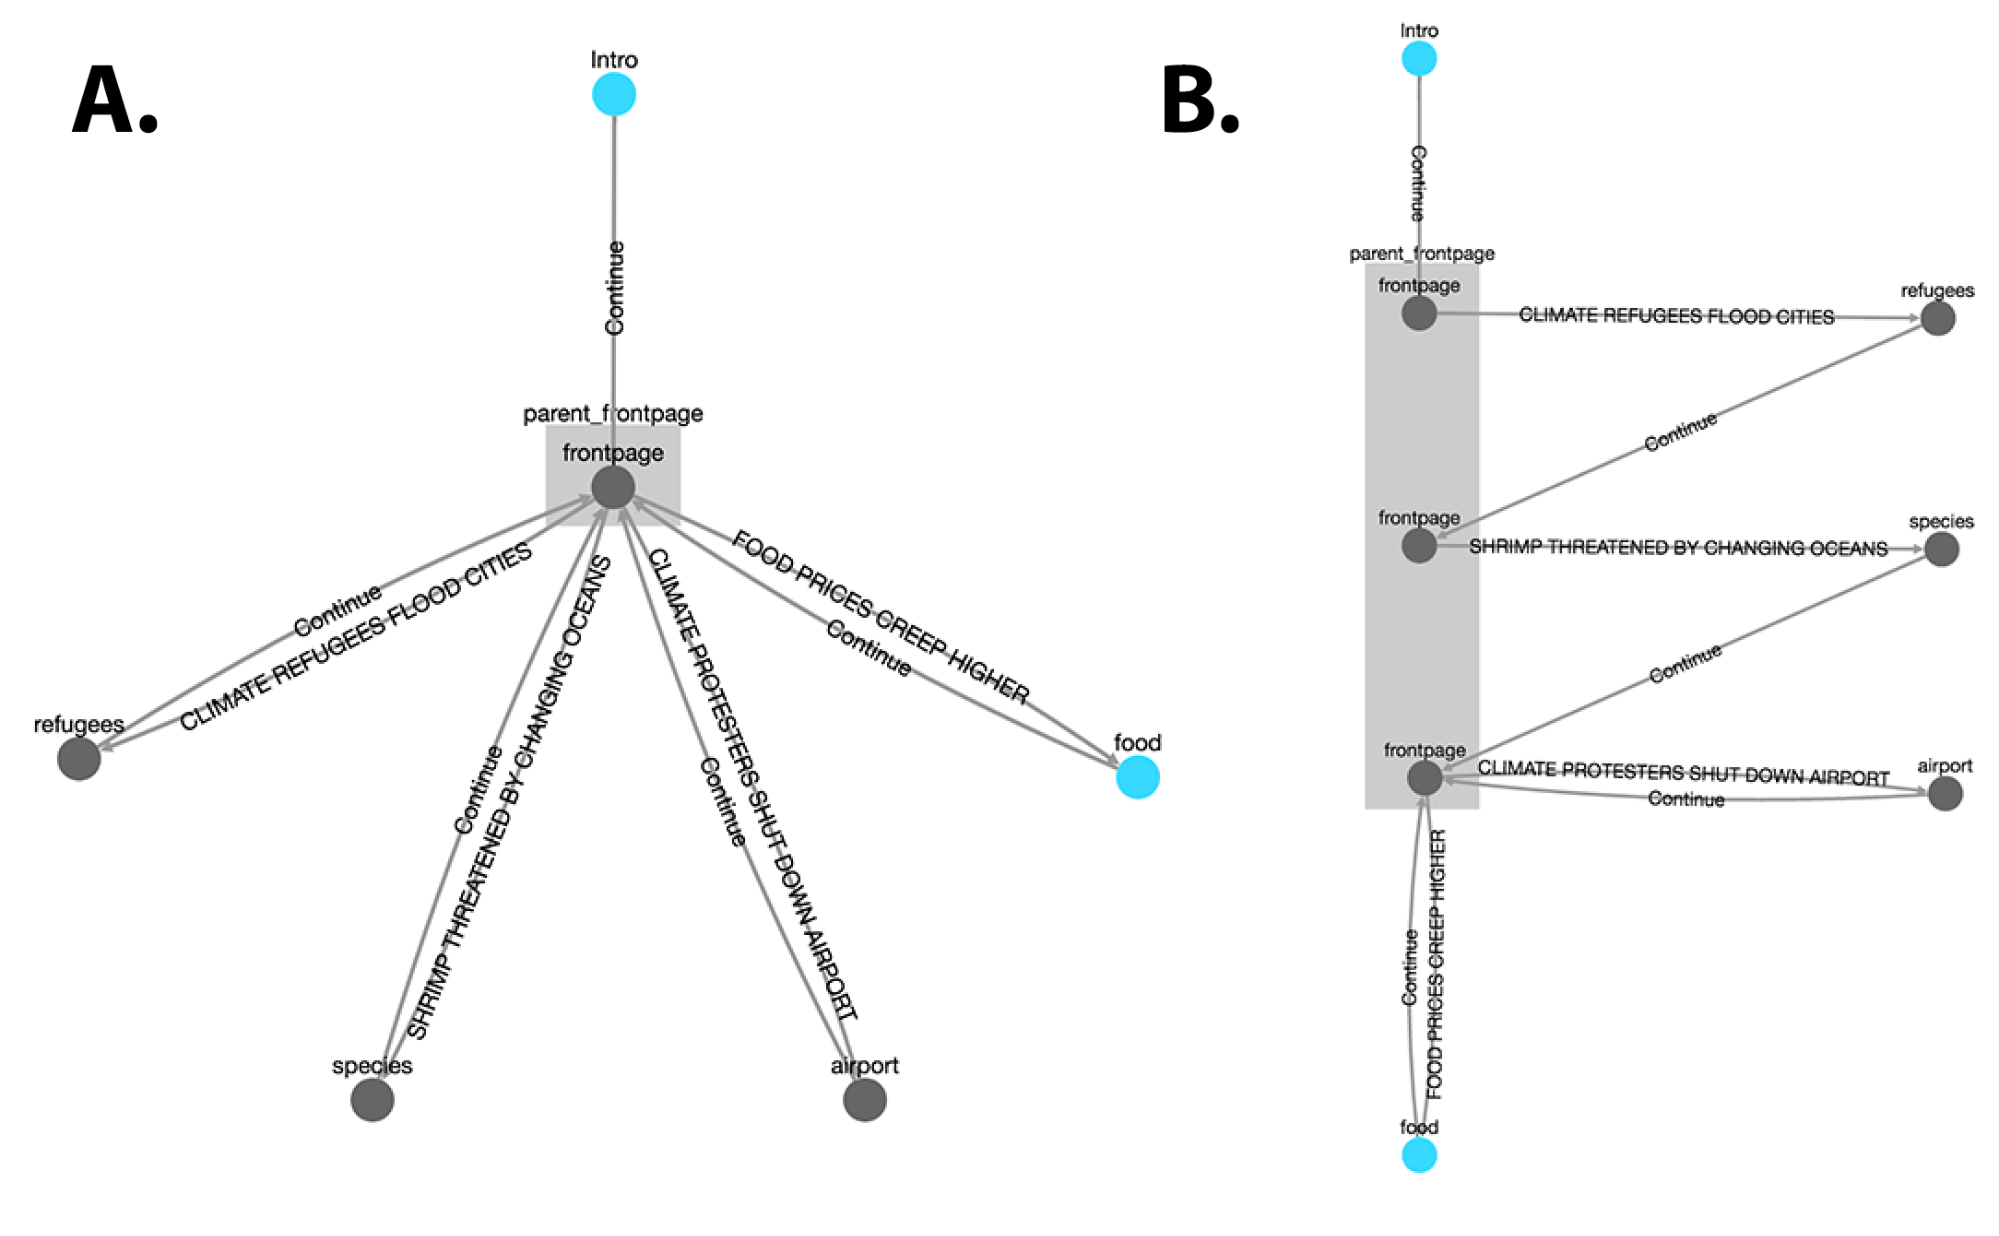
\includegraphics[width=\textwidth]{figures/3-StoryAssembler/viz1.png}
    \caption{Visualization with articlesRead as differentiating state value (B) and not (A).}
    \label{fig:viz}
\end{figure}

%%%%%%%%%%%% END FIGURE %%%%%%%%%%%%%%%%%%%%%%%%%%%%%%%%

In the visualization, we specify a subset of the narrative's state variables to establish whether a node in the structure could be considered structurally identical under different contexts. A good example is a short test segment where Emma is sitting in an airplane reading the newspaper. After an introduction (which fulfills an introductory goal element) she has a choice to read any of four articles, incrementing a state variable \texttt{articlesRead}. When four articles are read, the last goal element is fulfilled and the segment ends.

If we set the visualization to not consider \texttt{articlesRead} as a differentiating state value, we get a flower-like structure with the central node as the recurring fragment (Figure \ref{fig:viz}a). If we set \texttt{articlesRead} as a differentiating state value, however, we get a different structure (Figure \ref{fig:viz}b) where the recurring node, although identical in content, appears as a separate entry. However, they are still grouped together in a box, due to their shared content ID. This type of viz flexibility is desirable, as there are cases where authors may want to change what is considered a revisited node, in order to ensure the proper state changes are occurring. This may also be a good strategy to use in works where most of the dynamism results from state, and the viewer can toggle which variables are being considered to differentiate a node as unique.

%%%%%%%% BEGIN FIGURE %%%%%%%%%%%%%%%%%%%%%%%%%%%%%%%%%

\begin{figure}
    \centering
    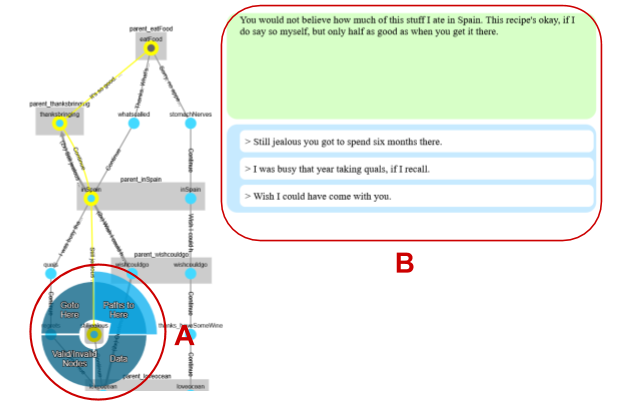
\includegraphics[width=\textwidth]{figures/3-StoryAssembler/viz2.png}
    \caption{When right-clicked, a node in the visualization brings up a contextual menu. Clicking ``paths to here" will highlight paths to this node in yellow (as shown), while also bringing up the narrative at that state (B). Valid and invalid nodes for this point of the story can also be shown.}
    \label{fig:viz2}
\end{figure}

%%%%%%%%%%%% END FIGURE %%%%%%%%%%%%%%%%%%%%%%%%%%%%%%%%

Blue nodes are used to signal when fragments are satisfying goal elements. Right-clicking nodes brings up a contextual menu (Figure \ref{fig:viz2}), allowing the viewer to highlight narrative paths through the diagram leading to this node. Additionally, the viewer can also use this menu to see which fragments were considered valid and invalid by StoryAssembler when it selected that fragment as the best fit in the progression. This was enormously useful for situations where the author has in mind a specific spot for a fragment, but it isn't currently being assembled there. They can right-click where a different node is selected, see the desired node, along with a listed state condition that failed, precluding its appearance.

Lastly, paths between nodes are aggregated into thicker lines in the case where multiple unique playthroughs traverse the same connection. This helps convey the scale of difference between main paths and unique side paths at a glance.

Because of these features, authors were able to locate out-of-place nodes in initial scene drafts quickly, and see if tweaks to those nodes (be that in conditions, effects, or some other detail) resulted in correct placement across many branches. It would also show when nodes were inadvertently orphaned by changes to other parts of the story (typically by modifying state the orphaned nodes depended on) thus saving time in some of the initial stages of scene composition.


\paragraph{Compound Fragment Authoring Patterns}

In the course of trying to navigate the particular challenges with compound fragments, we found that establishing abstract authoring patterns to copy and paste provided useful templates for writers to use. An example pattern can be seen in Figure \ref{fig:auth-pattern}, which allows for fragments to be available both as standalone beats (linked to another via a system-inserted ``continue" link) or by virtue of a ``linking choice label fragment", here seen as ``optionalChoiceLabel."

%%%%%%%% BEGIN FIGURE %%%%%%%%%%%%%%%%%%%%%%%%%%%%%%%%%

\begin{figure}
    \centering
    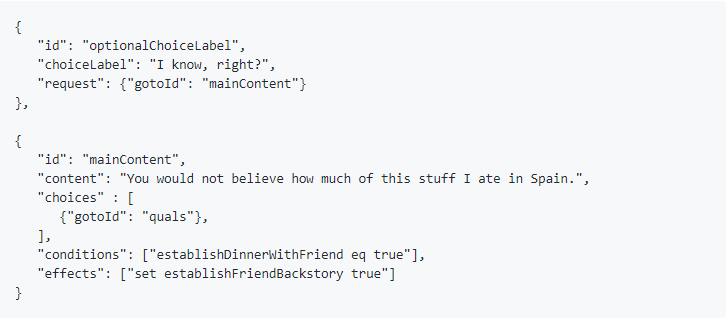
\includegraphics[width=\textwidth]{figures/3-StoryAssembler/data-object-1.png}
    \caption{A sample authoring pattern for a fragment which is available both through a choice (by way of the ``optionalChoiceLabel" fragment) and as a standalone fragment linked via ``Continue."}
    \label{fig:auth-pattern}
\end{figure}

%%%%%%%%%%%% END FIGURE %%%%%%%%%%%%%%%%%%%%%%%%%%%%%%%%

Of equal or more importance to these snippets themselves, was a paired summary of ``features and caveats" for each pattern. These ``gotchas" could frequently be unintuitive and difficult to remember, and were recurring stumbling blocks for content creation. For example, in the aforementioned pattern (due to vagaries of StoryAssembler's state evaluation system) an ``optional choice fragment" can't have effects that satisfy the main content fragment's preconditions. This is only something that would be apparent after much debugging and stepping through state logs, and not something in practice we would want our authors to have to deal with. Even describing the caveat at times could stretch a writer's ability to maintain clarity about what the fragment was enabling, but if nothing else it helped clarify system capabilities.

Over time, these system-specific patterns were aggregated in our ``writer's bible", which also contained a shorthand reference for the template syntax, dynamic goal element syntax, and other domain specific languages. The creation of such documents should be of high importance for complex dynamic narrative systems, as they pave the way for later efforts like opening up authoring to novice writers, or open sourcing the library. The writer's bible for StoryAssembler was cleaned up and formalized, and is currently available as part of its open-sourced library on Github \cite{github_storyassembler}.


\subsubsection{Controllability}

Because of our choice to pursue a narrative driven by conversation, we set up a situation with 
very high Contextuality. This in turn demands high Controllability, such that we don't generate juxapositions of content that don't make sense. This problem is compounded by the fact that, due to high Complexity, it's easy to write something in StoryAssembler with bad dynamics. This manifests itself as paths that, when traversed, result in a ``No Path Found" error, meaning the system cannot find any content that fulfills the current state conditions, while making progress towards the goal state. StoryAssembler has a boolean variable in its configuration for ``randomness" which forces it to, instead of picking the first top-scoring fragment assembly from the sorted list of possible assemblages, randomly pick from the multiple top-scoring assemblages, if their scores are identical. In very early prototypes of \textit{Emma's Journey}, however, it was so confusing and difficult to debug problems with bad content dynamics that we kept it turned off for the rest of the project, leaving it for some future date once we had the baseline content ``locked down."

This problem with complex state conditions isn't unique to StoryAssembler. Indeed, in many ways authors trade one set of problems for another when trying to systemically generate content rather than hand-author it. For example, Mawhorter noted when writing for Dunyazad stories that ``by limiting the complexity of vignettes and refreshing most of the world state between vignettes [...] the system has fewer opportunities to accidentally create plot holes" \cite{dunyazad}. However, for the task we set ourselves with \textit{Emma's Journey}, we wanted to confront the challenge directly, by pushing the complexity of individual scenes, and even having world state bleed over from one scene to the next.

When starting, our first instinct when confronting this Controllability problem was to apply strategies that normally work with systems like Twine or Ink. We thought we could first go through and write a static story graph for the scene, then go back through and slowly introduce complexity, until we reached a point where the scene's dynamicness and flexibility fulfilled our requirements (or at least until we'd exhausted our available time!).

In practice, this turned out not to be as feasible a plan as we'd hoped. Because StoryAssembler is greedily searching for fragments to fulfill goals, no matter the order, content added to increase dynamicity in one section of a narrative could break the progression in earlier parts of the scene because it technically satisfied a requirement earlier on. In reaction to this, our authors became proscriptive with state gating through flags or other variables. This uncomfortably echoes the same issues Tearse, Mawhorter, and Reed encountered when writing in Skald for \textit{Problem Planets}, where ALPs restricted the state so much, they were effectively pre-scripting the scenes.

Spierling and Szilas had a similar problem with authoring for their IDTension and Rencontre systems:

\begin{quote}
    Since it appears difficult to grasp the specifics of an engine, and therefore to ground any story design around the underlying computational models, some authors tended to use only a subpart of the engine's features. As a typical experience in first authoring
attempts with each of our engines, an author would naturally try to reduce the functionality to a linear or branching structure, which is more intuitive.
For example, the first story that was written with Rencontre by an author external to the project did not use fuzzy hypersections, which constitute one of the distinctive features of this engine. [...] In other words, the result was far from conversational storytelling. It rather resembled well-known structures of casual or adventure games \cite{authoring_issues}.
\end{quote}

There was a further problem that emerges from this. Even scene fragments that are ``dynamically linked through state" can be functionally static, if the conditions gating their appearance are only satisfiable in one way. Given the cognitive overhead of state tracking for dynamic links, authors could potentially cover ground faster by authoring several statically-linked fragments, as opposed to fewer (but more dynamic) fragments. This is the heart of the ``authoring wall" issue we introduced in Section \ref{authoring-wall}, where a dynamic unit of content that covers ten games states (but takes an hour to write) is ``slower" than ten units of static content that cover one state per piece and can all be written in half an hour.

For \textit{Emma's Journey}, we sought to get around this problem by splitting the authoring tasks into two types: structural design and implementation. As mentioned earlier, for each scene, we would go over the beats of content we wanted to be present. Then, we would come up with a structural framework to deliver that content. We would ``clump" content into more manageable segments (typically five or six per scene) and then think about how those clumps could be rearranged dynamically within the scene, while still retaining coherency.

After these sessions, we would make placeholder fragments (with no surface text, just descriptions) and link them together dynamically as we'd outlined in the diagram. Troubleshooting then could be confined purely to syntax errors and state errors, not things relating to surface text templating or other issues. The simple one-sentence descriptions for content would provide just enough context that if they appeared in strange places, it would be noticeable, but not so much that we would get distracted by trying to make transitions seamless.

After the fragments were in place and behaving correctly, we could then do a pass where writers would put in the text content, as well as the choice labels and other components. The final pass was for injecting more dynamism or smoothing transitions using state-based templating, or trying to add more choices to flesh out the dynamic core, even if said choices provisionally only had a few different ways they could link. At the least, they provided easy ``hooks" for returning later to add even more dynamism. The main focus of our design centered around increasing dynamism for the ``beats" satisfying the goal elements.

This tactic of structural design meetings up front also enabled us to divide labor between scene beats, and the capability to combine libraries of content between files meant that writers could then go off separately and create content to fulfill them, knowing what the other beats would be in the scene, and a rough idea of what they would entail. Writers could also coordinate on state changes they wanted to make in their section, and which variables were available for them to use to customize the state templating to make the text more reactive to player choice and gameplay. Then, a final editing pass was done once they brought their files together to smooth out rough edges.

\subsubsection{Authorability Summary}

The challenge set before us by \textit{Emma's Journey} was a steep one. While (from a technical format perspective) content creation for StoryAssembler is very similar to \textit{Ice-Bound}, the Proficiency required for the specific case of this project extended beyond software. It provided an exciting opportunity to head up a ``writer's room" of novice writers engaging with procedural authoring, with its own set of issues that comes from any project management endeavor. StoryAssembler's capabilities to enable collaboration between multiple writers on single scenes helped ease the pain points, but careful planning was still required from a narrative design standpoint, making this a medium Proficiency endeavor.

In comparison with \textit{Ice-Bound}, StoryAssembler's fragment construction driven by goal elements is far more complex to author for. Additionally, it has all the surface text templating complexities of \textit{Ice-Bound}, but also potentially applied to the goal state itself, in addition to the content. Therefore, on the standpoint of content authoring (excluding issues of narrative design) StoryAssembler has high Complexity.

Because we had high standards for the Contextuality of the narrative, and we chose to pursue a story mediated through character dialogue, we set ourselves a requirement for high Controllability. Many of the most pernicious problems writing for this system came from the juxtaposition of fragments with effects that would invalidate later fragments, meaning seemingly-innocuous changes could have outsize effects on the story as a whole.
%%GDoc comments%%
Navigating the proper arrangement of these fragments to satisfy goal elements, all while having to keep in mind changing variables affected by the mini-game, was very challenging. Additionally, we needed to push away from static linking (whether explicitly static by linking through id, or by implication through there only being one valid fulfillment of the state-driven call). While we tried to mitigate this with visualizations, their full development lies with future work. All these factors taken together gave StoryAssembler low Clarity. 
%%GDoc comments%%
We also found that StoryAssembler's ability to support both static and more dynamic authoring meant that, when hard-to-find narrative bugs manifest due to low Clarity, authors tend to reduce the procedurality of their story structures and link choices together statically just to ``get something reliably working''. Essentially, authors have a comfort zone for authorial Proficiency and Clarity, and will reduce content complexity to stay within that zone. Given that we wanted to push the dynamism as much as possible, this capitulation over time somewhat undermined the long-term dynamic goals of the project. Our JSON editor attempted to lower required Proficiency, and the visualization tried to increase Clarity, but tool enhancements were needed to reliably represent more complex structures in longer narratives, which is exactly where authors need the most support. For the editor, an example is the aforementioned issues with edge cases in complex fragments (with dynamic choices or content compounded from several nodes). For the viz, a particularly thorny example is how best to represent the traversal graph where the indexicality of each node (fragment) is very high, but differentiating between different cases of state-dependent linkages is very important.

In the future, this might be avoided by treating authoring requirements and system capabilities more as equal partners. For \textit{Emma's Journey}, it might have served better to balance complexity such that the authoring tools kept pace with system capabilities, rather than extending system capabilities beyond the reach of the authoring tools. While we did push the dynamism of the system a great deal, complex structures many times required extensive ``design debugging'' to ascertain why certain content was being displayed at certain times, which cut into time that could have been used to deepen the narrative content.

\textit{Emma's Journey} was a valiant first effort, but StoryAssembler is capable of even more complex narrative dynamics, \textit{if the clarity while authoring enables it}. These could enable potentially new experiences, but equally valid would be focusing work on better supporting the basic authoring patterns and capabilities, until such authoring becomes more tenable.

\subsection{Future Work}

After \textit{Emma's Journey} was finished and released, StoryAssembler was extracted from the game's codebase, and roughly formulated into an open source standalone JavaScript library \cite{github_storyassembler}. While functional, it's still in its early stages, with a few key expressive capabilities from \textit{Emma's Journey} left to be abstracted and formalized for reuse in other contexts. It's hoped that with further development it will become an attractive beachhead for practitioners seeking to tackle problems in a similar space.

Of particular interest is the further development of authoring tools similar in sophistication to the \textit{Ice-Bound} visualizations that could help increase Clarity for authoring with the system. StoryAssembler's capabilities have not yet been fully plumbed, and so the next ``technical push" in terms of the system must be for systemic authoring support tools, such that the unexplored capabilities can be leveraged for new types of interactive experiences.

In the realm of more wildly ambitious possibilities, the StoryAssembler system has been extracted while preserving the separation between the HTN-like planner system (internally called bestPath) and the general forward state-space planner that calls it. It may be possible, if the code is further segmented and abstracted, to ``substitute in" different algorithms to either of these systems, in order to even more widely explore its systemic dynamics, perhaps as more a platform for telling stories than an individual system. Integration of systems such as a javascript port of a Prolog interpreter or a JSHOP-style planner would enable intriguing new explorations, though they would undoubtedly come with their own content authoring complexities and concomitant issues.

\subsection{System Summary}

\textit{Emma's Journey} had ambitious desired features which set us up for a difficult authorial challenge. It was of \textbf{medium Explorability} and \textbf{medium Replayability}, because we wanted players to both be able to explore different states through performance with the mini-game, and also go back to try scenes multiple times to make different choices, or experiment with different starting conditions. Unfortunately, due to the \textbf{high Complexity} derived from the complex interplay between hierarchically-assembled fragments and the goal elements, we weren't able to reliably author fragments that were reusable across many different contexts, leaving us with \textbf{low Reusability}. Finally, the demands of the specific narrative format of \textit{Emma's Journey} meant that fragments needed to be tightly connected and avoid nonsensical juxtapositions. We did not have the benefit of a forgiving frame narrative as in \textit{Ice-Bound}. Therefore, we were setting ourselves up for a \textbf{very high Contextuality} requirement.

In order to meet this challenge, we tried to keep the proficiency requirement as low as possible. However, the choice to engage a team of writers, rather than two writers also doubling as system engineers as in \textit{Ice-Bound}, meant that our requirements for teamwork and collaborative narrative design pushed us to \textbf{medium Proficiency}. The expressiveness of the system, driven as it was by the various possible fragment assemblages and goal state possibilities, meant we also had a \textbf{high Complexity} problem. This was compounded by the emergent narrative dynamics, which made it difficult when adding content to predict how other content in the scene would then be assembled. We tried to ameliorate this through the use of some system-specific authoring patterns and an initial attempt at a visualization tool, but StoryAssembler remains a challenging system with \textbf{low Clarity}. Future work hopefully can develop these tools further, in order to enable authoring which can leverage its full potential.

\subsection{Next}

Despite the challenging hurdles \textit{Emma's Journey} presented, we were able to overcome them to offer a completed experimental research game which generates choice-driven narratives in concert with generated mini-games, all working together to create a unified, compelling experience.

Both \textit{Ice-Bound} and StoryAssembler were combinatoric, leveraging their systems in a similar approach to juxtapose content together based on pre-condition logic and blackboard state, though the final expression of that form (and how that juxtaposition was controlled) differed greatly.

However, what if one could take such approaches, but apply the combinatorics to ``pattern match" to a simulation of already existing events? And what if one pushed on that symbolic connection between simulation and narrative representation, to make even the connection itself  something which could be procedurally manipulated?

This is the motivating premise of the final group of prospective systems and prototypes, each an exploration of a similar approach, using a different methodology: \textit{LegendWriter}, \textit{Argosy}, and \textit{Delve}.
